\documentclass[aspectratio=169]{beamer}

\usepackage{tikz}
\usepackage{pgfplots}
\usetikzlibrary {positioning,shapes.misc}
\usepackage[ruled,linesnumbered,boxed]{algorithm2e}
\usepackage{float}

\def\input#1{\fbox{#1}} % draft mode

\usecolortheme{beaver}
\title{Stage-Based Strategy for Scheduling Jobs Problem with Max-Min Fairness}
\subtitle{Project for Algorithm and Complexity }
\author{Taoran Han, Longxuan Wei, Zilong Li}
\institute{Department of Computer Science, \\ Shanghai Jiao Tong University, Shanghai, China}
\begin{document}
\maketitle

\AtBeginPart{\frame{\partpage}\frame{\tableofcontents}}

% Part 1: Design
\part{Algorithm Design}
\section{Introduction}
\begin{frame}
\frametitle{Introduction} % 幻灯片标题
% With the rapid growth on the scale of data clusters, there are more and more data online in different Geo-Distributed Data Centers. And the amount of data is so big that it is a emerging demand to schedule data within the bandwidth across data centers and take advantage of data locality at the same time. Moreover, the workload of computational resources requires to be distributed as fair as possible, in order to balance the cost in different areas.
\begin{figure}[h]
    \centering
    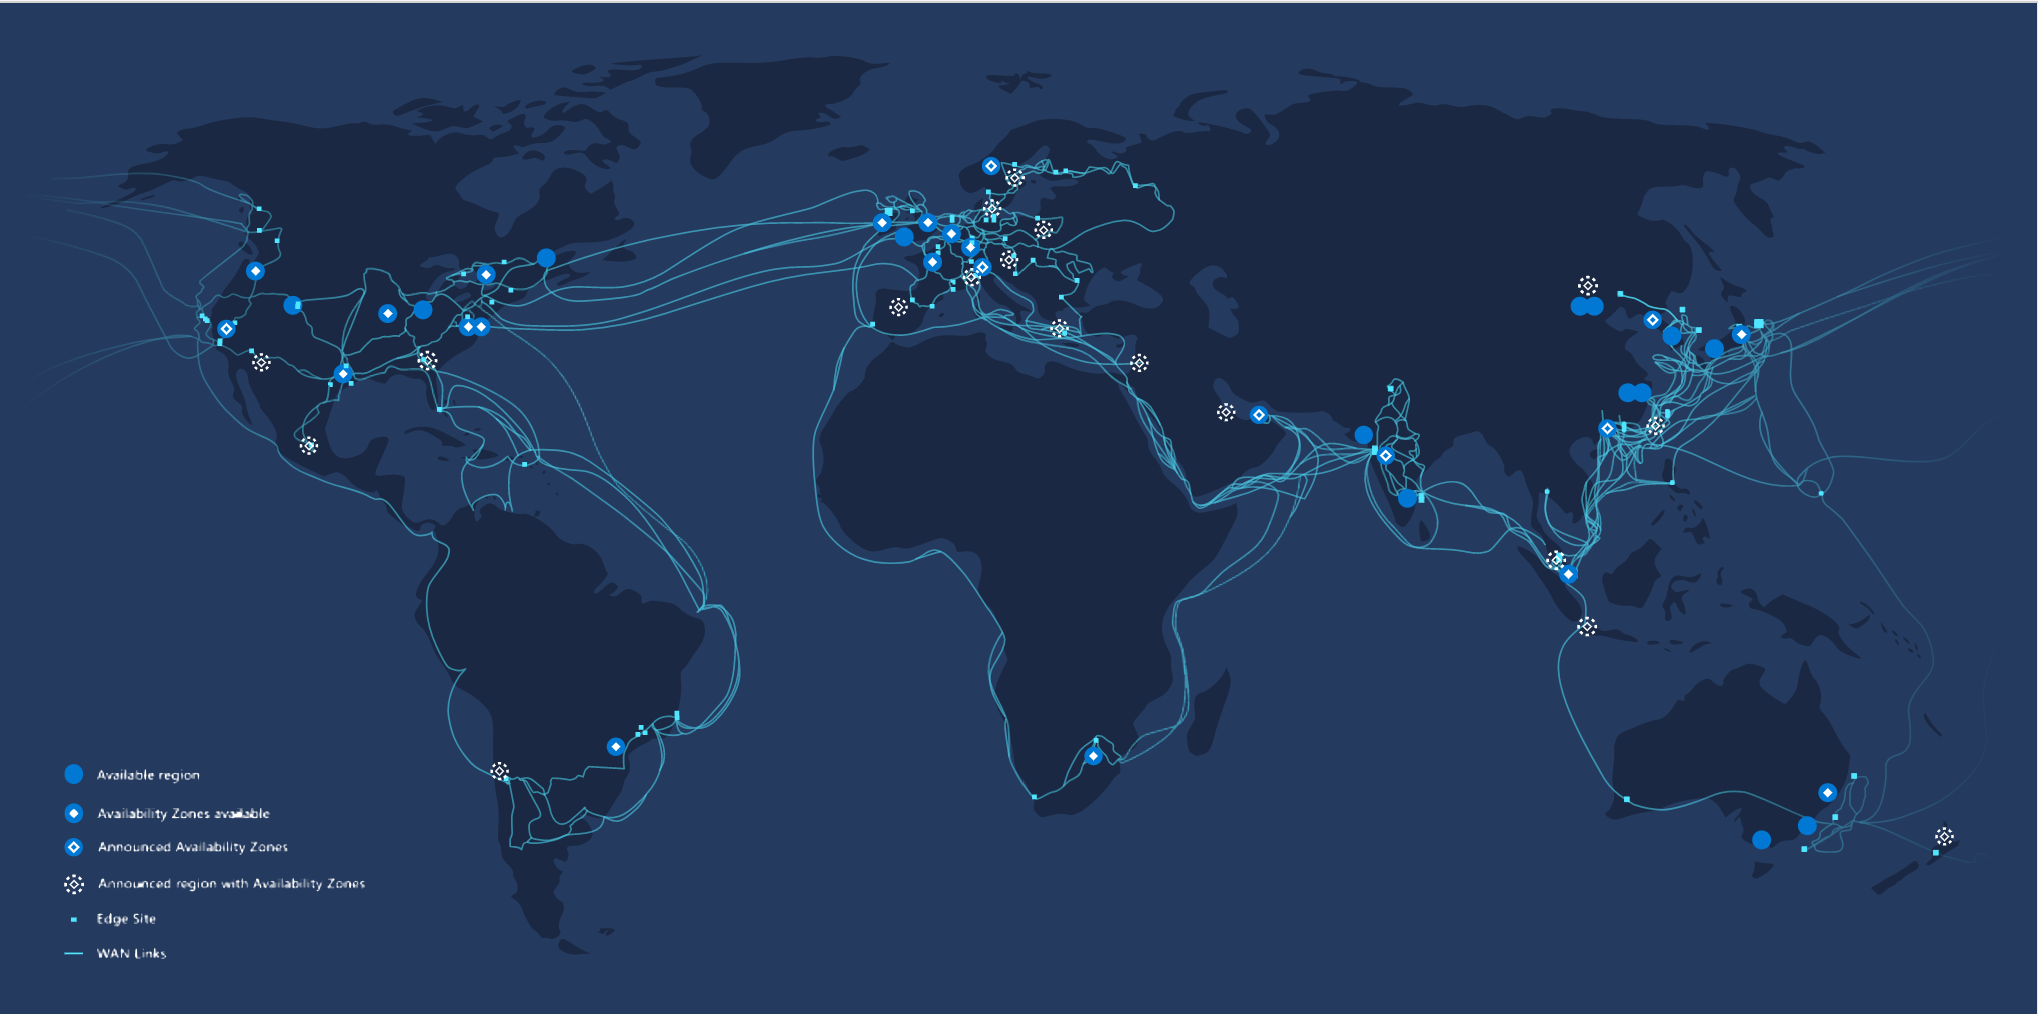
\includegraphics[width=0.9\textwidth]{img/network.png}
    \caption{Data centers and its connection in Azure global network\cite{azure}}
    \label{fig:azure}
\end{figure}
\end{frame}

\begin{frame}
\frametitle{Notation}
\begin{table}[h]
    \centering\scriptsize
    \caption{Symbel Table of Variables for Scheduling Jobs Problem}\label{tab:variables}
    \begin{tabular}{c|l}
    \hline
         Variable & Meaning\\
    \hline
        $K$ & The number of jobs\\
        $m$ & The number of data centers\\
        $t_k$ & The number of tasks of job $k$\\
        $s_i$ & The number of slots of center $i$\\
        $e_{k,i}$ & The execution time of task $i$ of job $k$\\
        $b_{i,j}$ & The bandwidth from center $i$ to center $j$\\
        $d_{k,i}^j$ & The amount of data that task $i$ of job $k$ requires from center $j$\\
        $T_{i,j}^k$ & The amount of data that task $j$ of job $k$ requires from task $i$ of job $k$\\
        $q_k$ & The number of stages of job$k$\\
        $p_i^k$ & The number of tasks of stage $i$ of job $k$\\
        $x_{k,i}^j$ & Whether task $i$ of job $k$ is allocated to center $j$\\
        $c_{k,i}$ & The completion time of task $i$ of job $k$\\
        $C_k$ & The completion time of job $k$\\
        $ACT$ & The average completion time of all jobs\\
    \hline
    \end{tabular}
\end{table}
\end{frame}

\begin{frame}
    
\end{frame}


% Part 2: NPC
\part{NP-Completeness}
\section{Proof method}
\begin{frame}[allowframebreaks=0.8]
\frametitle{proof}
    The problem is to schedule all the tasks in the DAG to a number of worker nodes --- while minimizing the average time of the job.
    
    To prove this, we need to reduce in to a similar and known NPC problem, which is the 3-SAT problem. Because that the max-min fairness is a condition which is to optimize the result after finding out a result. And this does not affect the judgment of NPC, so it is not mentioned in the process of proof.
\end{frame}


% Part 3: Algorithm
\part{Algorithm \& Test}
\section{Algorithm \& Complexity}

\begin{frame}[allowframebreaks=0.8]
\frametitle{Floyd-Warshall on Bandwidth}
    We can calculate the corresponding bandwidth between every two data centers. Considering that the data transferring path need to be optimal (the data could be transferred indirectly), we will use the Floyd-Warshall's Algorithm. 
    
    This assumption could be justified by the fact that we could construct a \empty{transfer} task without the need for any computing resources to pass the data from the previous transfer. Because data could transfer on every link, the data could also been transferred indirectly in this way.
    
    \begin{figure}
        \centering
        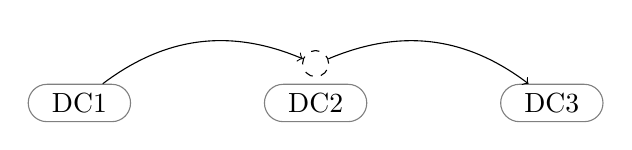
\begin{tikzpicture}[node distance=1cm]
\tikzstyle{dc} = [rounded rectangle,draw=gray,text centered,text width=1cm];
\node[dc] (v1) at (-1,0.5) {DC1};
\node[dc] (v2) at (2,0.5) {DC2};
\node [dc] (v3) at (5,0.5) {DC3};
\node[circle,radius=1cm,draw,dashed] (v4) at (2,1) {};
\draw  (v1) edge[->,bend left] (v4);
\draw  (v4) edge[->,bend left] (v3);
\end{tikzpicture}

        \caption{Indirect transfer through a \emph{transfer} task}
        \label{fig:my_label}
    \end{figure}
    
    The reciprocal of the bandwidth is the transfer time through this line. And the bandwidth could be calculated reversely after the process of Floyd-Warshall.
    
    \begin{equation*}
        \frac{1}{b_{i,j}}\rightarrow \textbf{\fbox{Floyd-Warshall}} \rightarrow \frac{1}{b^\prime_{i,j}}
    \end{equation*}
    
    The Floyd-Warshall's Algorithm on the bandwidth matrix costs $O(m^3)$, where $m$ is the number of data centers.
\end{frame}

\begin{frame}
\frametitle{DAG Stage Seperation}

\begin{algorithm}[H]
\caption{DAG Stage Separation}
\KwIn{Request Matrix $D$}
\KwOut{Stage Separation for every job}
Reduce $D$ to $D^\prime$ with task items only\;
Turn $D^\prime$ into adjacency list $G$ on positive element\;
Get topological order of $G$ by recording to \textsc{PRE} of Depth-First Search\;
Run Breadth-First Search on $G$ in topological order to get the stage level, updating the level in a top-down method\;
Group task by (job, level)\;
\end{algorithm}
The algorithm is efficient on sparse graph with the use of adjacency list, with the total running time of $O(|V|^2+|E|)$. In this case, $|E|=\Theta(|V|)$, thus $O(|V|^2)$ is the time complexity in this stage, where $|V|=\# tasks=\sum_{k=1}^K\sum_{i=1}^{t_k}1$ is the number of all tasks.
\end{frame}

\begin{frame}[allowframebreaks=0.8]
\frametitle{Improvement on \texttt{max}}
It is discovered that using built-in function \texttt{max} in CPLEX is \emph{slow}. We turned the max function into inequalities. 

\begin{align}
    c_{k,i} &\geq t_{k,i} + e_{k,i} \label{eq:t1}\\
    c_{k,i} &\geq t_{k,i}^\prime + e_{k,i} \label{eq:t2}\\
    t_{k,i} &\geq \sum_{j_1=1}^m \frac{x_{k,i}^{j_1}\times d_{k,i}^{j_2}}{b_{j_2,j_1}},&& \forall 1\leq j_2\leq m\\
    t_{k,i}^\prime &\geq \sum_{j_1=1}^m\sum_{j_2=1}^m \frac{x_{k,i}^{j_1}\times x_{k,j_3}^{j_2}\times T_{j_3,i}^k}{b_{j_2,j_1}} + e_{k,i},&& \forall 1\leq j_3\leq t_k\label{eq:tend}
\end{align}

It is obvious that to optimze the average cost, $c_{k,i}$ is required to touch the tightest bound in Constraints \eqref{eq:t1} and \eqref{eq:t2}, which satisfies the original equality of \eqref{eq:taske}.

Assume that $c^\prime_{k,s}$ is the cost of stage $s$ in job $k$, then it is the longest cost among all tasks in this stage. And Equation \eqref{eq:stage} is turned into
\begin{align}
    C_k &= \sum_{s=1}^{q_k} c^{\prime}_{k,s} \label{eq:jobm1}\\
    c^\prime_{k,s} &\geq c_{k,i},\quad \forall i: 1+\sum_{l=1}^{s-1} p_{l}^k \leq i \leq \sum_{l=1}^{s} p_{l}^k \label{eq:jobm2}
\end{align}
since the task in every stage could be non-continuous, it is just a representation to show that it is the maximum elapsed time in every stage.
\end{frame}

\begin{frame}
\frametitle{Iterative Max-Min Fairness}

\begin{algorithm}[H]
    \caption{Iterative Max-Min Fairness Algorithm}
    Initialize Optimize Model with basic constraints \eqref{eq:one}, (\ref{eq:t1} -- \ref{eq:tend}), (\ref{eq:jobm1} -- \ref{eq:jobm2})\;
    \texttt{ConstrSlot} $\leftarrow$ []\;
    \Repeat{
        original Constraint \eqref{eq:slot} is satisfied
    }{
    \ForEach{\emph{slot}}{
        \eIf{\emph{slot}$\in$\texttt{ConstrSlot}}{
        add constraint on mono \emph{slot} similar to Constraint \eqref{eq:slot}\;
        }
        {
        fix the allocated task on \emph{slot}. }
        Optimize Model\;
        append the overflow slots to \texttt{ConstrSlot}\;
        }
    }
\end{algorithm}
\end{frame}

\begin{frame}
    As a result, the total time complexity of our algorithm is:
\begin{equation*}
    O(m^3)+O(n)+O(mT)
\end{equation*}
where $n=\#tasks$. Our algorithm performs less than 10s on Toy Data.
\end{frame}

\section{Test on Toy Data}

\begin{frame}
\frametitle{Toy Data (without max-min)}
    \begin{figure}[h]
    \centering
    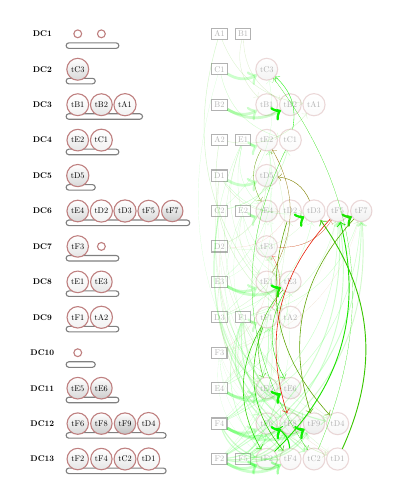
\begin{tikzpicture}[scale=0.3,every node/.style={scale=0.3}]

\tikzstyle{dc} = [rounded rectangle,right,draw=gray,yshift=-0.5cm];
\tikzstyle{task} = [circle,draw=red!50!black!50,top color=white];
\tikzstyle{dp}=[draw,opacity=0.3]
\node[font=\bfseries] at (-1.5,0) {DC1};
\node[dc,text width=2.0cm] (DC1) at (-0.5,0) {};
\node[dp] (A1) at (6,0) {A1};
\node[dp] (B1) at (7,0) {B1};
\node[task] at (0,0) {};
\node[task] at (1,0) {};
\node[font=\bfseries] at (-1.5,-1.5) {DC2};
\node[dc,text width=1.0cm] (DC2) at (-0.5,-1.5) {};
\node[dp] (C1) at (6,-1.5) {C1};
\node[task,bottom color=black!15.0] at (0,-1.5) {tC3};
\node[task,bottom color=black!15.0,opacity=0.3] (tC3) at (8,-1.5) {tC3};
\node[font=\bfseries] at (-1.5,-3.0) {DC3};
\node[dc,text width=3.0cm] (DC3) at (-0.5,-3.0) {};
\node[dp] (B2) at (6,-3.0) {B2};
\node[task,bottom color=black!5.0] at (0,-3.0) {tB1};
\node[task,bottom color=black!5.0,opacity=0.3] (tB1) at (8,-3.0) {tB1};
\node[task,bottom color=black!10.0] at (1,-3.0) {tB2};
\node[task,bottom color=black!10.0,opacity=0.3] (tB2) at (9,-3.0) {tB2};
\node[task,bottom color=black!5.0] at (2,-3.0) {tA1};
\node[task,bottom color=black!5.0,opacity=0.3] (tA1) at (10,-3.0) {tA1};
\node[font=\bfseries] at (-1.5,-4.5) {DC4};
\node[dc,text width=2.0cm] (DC4) at (-0.5,-4.5) {};
\node[dp] (A2) at (6,-4.5) {A2};
\node[dp] (E1) at (7,-4.5) {E1};
\node[task,bottom color=black!10.0] at (0,-4.5) {tE2};
\node[task,bottom color=black!10.0,opacity=0.3] (tE2) at (8,-4.5) {tE2};
\node[task,bottom color=black!5.0] at (1,-4.5) {tC1};
\node[task,bottom color=black!5.0,opacity=0.3] (tC1) at (9,-4.5) {tC1};
\node[font=\bfseries] at (-1.5,-6.0) {DC5};
\node[dc,text width=1.0cm] (DC5) at (-0.5,-6.0) {};
\node[dp] (D1) at (6,-6.0) {D1};
\node[task,bottom color=black!15.0] at (0,-6.0) {tD5};
\node[task,bottom color=black!15.0,opacity=0.3] (tD5) at (8,-6.0) {tD5};
\node[font=\bfseries] at (-1.5,-7.5) {DC6};
\node[dc,text width=5.0cm] (DC6) at (-0.5,-7.5) {};
\node[dp] (C2) at (6,-7.5) {C2};
\node[dp] (E2) at (7,-7.5) {E2};
\node[task,bottom color=black!15.0] at (0,-7.5) {tE4};
\node[task,bottom color=black!15.0,opacity=0.3] (tE4) at (8,-7.5) {tE4};
\node[task,bottom color=black!5.0] at (1,-7.5) {tD2};
\node[task,bottom color=black!5.0,opacity=0.3] (tD2) at (9,-7.5) {tD2};
\node[task,bottom color=black!10.0] at (2,-7.5) {tD3};
\node[task,bottom color=black!10.0,opacity=0.3] (tD3) at (10,-7.5) {tD3};
\node[task,bottom color=black!15.0] at (3,-7.5) {tF5};
\node[task,bottom color=black!15.0,opacity=0.3] (tF5) at (11,-7.5) {tF5};
\node[task,bottom color=black!20.0] at (4,-7.5) {tF7};
\node[task,bottom color=black!20.0,opacity=0.3] (tF7) at (12,-7.5) {tF7};
\node[font=\bfseries] at (-1.5,-9.0) {DC7};
\node[dc,text width=2.0cm] (DC7) at (-0.5,-9.0) {};
\node[dp] (D2) at (6,-9.0) {D2};
\node[task,bottom color=black!10.0] at (0,-9.0) {tF3};
\node[task,bottom color=black!10.0,opacity=0.3] (tF3) at (8,-9.0) {tF3};
\node[task] at (1,-9.0) {};
\node[font=\bfseries] at (-1.5,-10.5) {DC8};
\node[dc,text width=2.0cm] (DC8) at (-0.5,-10.5) {};
\node[dp] (E3) at (6,-10.5) {E3};
\node[task,bottom color=black!5.0] at (0,-10.5) {tE1};
\node[task,bottom color=black!5.0,opacity=0.3] (tE1) at (8,-10.5) {tE1};
\node[task,bottom color=black!10.0] at (1,-10.5) {tE3};
\node[task,bottom color=black!10.0,opacity=0.3] (tE3) at (9,-10.5) {tE3};
\node[font=\bfseries] at (-1.5,-12.0) {DC9};
\node[dc,text width=2.0cm] (DC9) at (-0.5,-12.0) {};
\node[dp] (D3) at (6,-12.0) {D3};
\node[dp] (F1) at (7,-12.0) {F1};
\node[task,bottom color=black!5.0] at (0,-12.0) {tF1};
\node[task,bottom color=black!5.0,opacity=0.3] (tF1) at (8,-12.0) {tF1};
\node[task,bottom color=black!5.0] at (1,-12.0) {tA2};
\node[task,bottom color=black!5.0,opacity=0.3] (tA2) at (9,-12.0) {tA2};
\node[font=\bfseries] at (-1.5,-13.5) {DC10};
\node[dc,text width=1.0cm] (DC10) at (-0.5,-13.5) {};
\node[dp] (F3) at (6,-13.5) {F3};
\node[task] at (0,-13.5) {};
\node[font=\bfseries] at (-1.5,-15.0) {DC11};
\node[dc,text width=2.0cm] (DC11) at (-0.5,-15.0) {};
\node[dp] (E4) at (6,-15.0) {E4};
\node[task,bottom color=black!15.0] at (0,-15.0) {tE5};
\node[task,bottom color=black!15.0,opacity=0.3] (tE5) at (8,-15.0) {tE5};
\node[task,bottom color=black!20.0] at (1,-15.0) {tE6};
\node[task,bottom color=black!20.0,opacity=0.3] (tE6) at (9,-15.0) {tE6};
\node[font=\bfseries] at (-1.5,-16.5) {DC12};
\node[dc,text width=4.0cm] (DC12) at (-0.5,-16.5) {};
\node[dp] (F4) at (6,-16.5) {F4};
\node[task,bottom color=black!15.0] at (0,-16.5) {tF6};
\node[task,bottom color=black!15.0,opacity=0.3] (tF6) at (8,-16.5) {tF6};
\node[task,bottom color=black!20.0] at (1,-16.5) {tF8};
\node[task,bottom color=black!20.0,opacity=0.3] (tF8) at (9,-16.5) {tF8};
\node[task,bottom color=black!25.0] at (2,-16.5) {tF9};
\node[task,bottom color=black!25.0,opacity=0.3] (tF9) at (10,-16.5) {tF9};
\node[task,bottom color=black!10.0] at (3,-16.5) {tD4};
\node[task,bottom color=black!10.0,opacity=0.3] (tD4) at (11,-16.5) {tD4};
\node[font=\bfseries] at (-1.5,-18.0) {DC13};
\node[dc,text width=4.0cm] (DC13) at (-0.5,-18.0) {};
\node[dp] (F2) at (6,-18.0) {F2};
\node[dp] (F5) at (7,-18.0) {F5};
\node[task,bottom color=black!10.0] at (0,-18.0) {tF2};
\node[task,bottom color=black!10.0,opacity=0.3] (tF2) at (8,-18.0) {tF2};
\node[task,bottom color=black!10.0] at (1,-18.0) {tF4};
\node[task,bottom color=black!10.0,opacity=0.3] (tF4) at (9,-18.0) {tF4};
\node[task,bottom color=black!10.0] at (2,-18.0) {tC2};
\node[task,bottom color=black!10.0,opacity=0.3] (tC2) at (10,-18.0) {tC2};
\node[task,bottom color=black!5.0] at (3,-18.0) {tD1};
\node[task,bottom color=black!5.0,opacity=0.3] (tD1) at (11,-18.0) {tD1};
\draw[red!3.75!green,line width=1.0pt] (tB1) edge[->,bend right] (tB2);
\draw[red!12.15!green,line width=0.09259259259259259pt] (tC1) edge[->,bend right] (tC2);
\draw[red!6.0!green,line width=0.125pt] (tC1) edge[->,bend right] (tC3);
\draw[red!11.75!green,line width=0.06382978723404255pt] (tC2) edge[->,bend right] (tC3);
\draw[red!22.5!green,line width=0.3333333333333333pt] (tD1) edge[->,bend right] (tD3);
\draw[red!7.5!green,line width=1.0pt] (tD2) edge[->,bend right] (tD3);
\draw[red!36.0!green,line width=0.20833333333333334pt] (tD2) edge[->,bend right] (tD4);
\draw[red!50.0!green,line width=0.15pt] (tD3) edge[->,bend right] (tD5);
\draw[red!56.25!green,line width=0.1pt] (tE1) edge[->,bend right] (tE2);
\draw[red!3.0!green,line width=1.0pt] (tE1) edge[->,bend right] (tE3);
\draw[red!37.5!green,line width=0.1pt] (tE2) edge[->,bend right] (tE4);
\draw[red!23.625!green,line width=0.14285714285714285pt] (tE3) edge[->,bend right] (tE5);
\draw[red!13.125!green,line width=0.14285714285714285pt] (tE3) edge[->,bend right] (tE6);
\draw[red!6.75!green,line width=1.0pt] (tE5) edge[->,bend right] (tE6);
\draw[red!18.0!green,line width=0.20833333333333334pt] (tF1) edge[->,bend right] (tF2);
\draw[red!92.10000000000001!green,line width=0.048859934853420196pt] (tF1) edge[->,bend right] (tF3);
\draw[red!18.0!green,line width=0.20833333333333334pt] (tF1) edge[->,bend right] (tF4);
\draw[red!11.25!green,line width=0.3333333333333333pt] (tF2) edge[->,bend right] (tF5);
\draw[red!78.75000000000001!green,line width=0.07142857142857142pt] (tF3) edge[->,bend right] (tF5);
\draw[red!8.1!green,line width=0.4166666666666667pt] (tF4) edge[->,bend right] (tF6);
\draw[red!11.25!green,line width=1.0pt] (tF5) edge[->,bend right] (tF7);
\draw[red!90.0!green,line width=0.20833333333333334pt] (tF5) edge[->,bend right] (tF8);
\draw[red!1.875!green,line width=1.0pt] (tF6) edge[->,bend right] (tF8);
\draw[red!36.0!green,line width=0.20833333333333334pt] (tF7) edge[->,bend right] (tF9);
\draw[red!7.5!green,line width=1.0pt] (tF8) edge[->,bend right] (tF9);
\draw[opacity=0.2,red!25.0!green,line width=0.125pt] (A1) edge[->,bend right] (tA1);
\draw[opacity=0.2,red!25.0!green,line width=0.15pt] (A2) edge[->,bend right] (tA1);
\draw[opacity=0.2,red!16.875!green,line width=0.18518518518518517pt] (A1) edge[->,bend right] (tA2);
\draw[opacity=0.2,red!22.5!green,line width=0.16666666666666666pt] (A2) edge[->,bend right] (tA2);
\draw[opacity=0.2,red!30.0!green,line width=0.125pt] (B1) edge[->,bend right] (tB1);
\draw[opacity=0.2,red!3.75!green,line width=1.0pt] (B2) edge[->,bend right] (tB1);
\draw[opacity=0.2,red!33.33333333333333!green,line width=0.125pt] (B1) edge[->,bend right] (tB2);
\draw[opacity=0.2,red!6.25!green,line width=1.0pt] (B2) edge[->,bend right] (tB2);
\draw[opacity=0.2,red!7.8125!green,line width=0.13333333333333333pt] (C1) edge[->,bend right] (tC1);
\draw[opacity=0.2,red!5.0!green,line width=0.20833333333333334pt] (C2) edge[->,bend right] (tC1);
\draw[opacity=0.2,red!0.0!green,line width=0.06097560975609756pt] (C1) edge[->,bend right] (tC2);
\draw[opacity=0.2,red!3.5000000000000004!green,line width=0.4166666666666667pt] (C2) edge[->,bend right] (tC2);
\draw[opacity=0.2,red!0.625!green,line width=1.0pt] (C1) edge[->,bend right] (tC3);
\draw[opacity=0.2,red!0.0!green,line width=0.07894736842105263pt] (C2) edge[->,bend right] (tC3);
\draw[opacity=0.2,red!21.666666666666668!green,line width=0.09615384615384616pt] (D1) edge[->,bend right] (tD1);
\draw[opacity=0.2,red!68.33333333333333!green,line width=0.06097560975609756pt] (D2) edge[->,bend right] (tD1);
\draw[opacity=0.2,red!30.0!green,line width=0.20833333333333334pt] (D3) edge[->,bend right] (tD1);
\draw[opacity=0.2,red!33.33333333333333!green,line width=0.125pt] (D1) edge[->,bend right] (tD2);
\draw[opacity=0.2,red!87.50000000000001!green,line width=0.07142857142857142pt] (D2) edge[->,bend right] (tD2);
\draw[opacity=0.2,red!16.25!green,line width=0.1282051282051282pt] (D3) edge[->,bend right] (tD2);
\draw[opacity=0.2,red!0.0!green,line width=0.125pt] (D1) edge[->,bend right] (tD3);
\draw[opacity=0.2,red!14.583333333333334!green,line width=0.07142857142857142pt] (D2) edge[->,bend right] (tD3);
\draw[opacity=0.2,red!0.0!green,line width=0.1282051282051282pt] (D3) edge[->,bend right] (tD3);
\draw[opacity=0.2,red!26.666666666666668!green,line width=0.078125pt] (D1) edge[->,bend right] (tD4);
\draw[opacity=0.2,red!0.0!green,line width=0.05319148936170212pt] (D2) edge[->,bend right] (tD4);
\draw[opacity=0.2,red!5.0!green,line width=0.4166666666666667pt] (D3) edge[->,bend right] (tD4);
\draw[opacity=0.2,red!0.0!green,line width=1.0pt] (D1) edge[->,bend right] (tD5);
\draw[opacity=0.2,red!25.0!green,line width=0.16666666666666666pt] (D2) edge[->,bend right] (tD5);
\draw[opacity=0.2,red!0.0!green,line width=0.06912442396313365pt] (D3) edge[->,bend right] (tD5);
\draw[opacity=0.2,red!13.333333333333334!green,line width=0.09375pt] (E1) edge[->,bend right] (tE1);
\draw[opacity=0.2,red!22.22222222222222!green,line width=0.075pt] (E2) edge[->,bend right] (tE1);
\draw[opacity=0.2,red!2.5!green,line width=1.0pt] (E3) edge[->,bend right] (tE1);
\draw[opacity=0.2,red!0.0!green,line width=0.14285714285714285pt] (E4) edge[->,bend right] (tE1);
\draw[opacity=0.2,red!0.0!green,line width=1.0pt] (E1) edge[->,bend right] (tE2);
\draw[opacity=0.2,red!9.0!green,line width=0.20833333333333334pt] (E2) edge[->,bend right] (tE2);
\draw[opacity=0.2,red!0.0!green,line width=0.1pt] (E3) edge[->,bend right] (tE2);
\draw[opacity=0.2,red!22.499999999999996!green,line width=0.11111111111111112pt] (E4) edge[->,bend right] (tE2);
\draw[opacity=0.2,red!6.666666666666667!green,line width=0.09375pt] (E1) edge[->,bend right] (tE3);
\draw[opacity=0.2,red!0.0!green,line width=0.075pt] (E2) edge[->,bend right] (tE3);
\draw[opacity=0.2,red!1.0416666666666665!green,line width=1.0pt] (E3) edge[->,bend right] (tE3);
\draw[opacity=0.2,red!0.0!green,line width=0.14285714285714285pt] (E4) edge[->,bend right] (tE3);
\draw[opacity=0.2,red!0.0!green,line width=0.1pt] (E1) edge[->,bend right] (tE4);
\draw[opacity=0.2,red!3.3333333333333335!green,line width=1.0pt] (E2) edge[->,bend right] (tE4);
\draw[opacity=0.2,red!0.0!green,line width=0.05pt] (E3) edge[->,bend right] (tE4);
\draw[opacity=0.2,red!0.0!green,line width=0.05263157894736843pt] (E4) edge[->,bend right] (tE4);
\draw[opacity=0.2,red!0.0!green,line width=0.10344827586206896pt] (E1) edge[->,bend right] (tE5);
\draw[opacity=0.2,red!0.0!green,line width=0.06912442396313365pt] (E2) edge[->,bend right] (tE5);
\draw[opacity=0.2,red!23.333333333333332!green,line width=0.14285714285714285pt] (E3) edge[->,bend right] (tE5);
\draw[opacity=0.2,red!3.75!green,line width=1.0pt] (E4) edge[->,bend right] (tE5);
\draw[opacity=0.2,red!10.069444444444445!green,line width=0.10344827586206896pt] (E1) edge[->,bend right] (tE6);
\draw[opacity=0.2,red!0.0!green,line width=0.06912442396313365pt] (E2) edge[->,bend right] (tE6);
\draw[opacity=0.2,red!0.0!green,line width=0.14285714285714285pt] (E3) edge[->,bend right] (tE6);
\draw[opacity=0.2,red!0.0!green,line width=1.0pt] (E4) edge[->,bend right] (tE6);
\draw[opacity=0.2,red!6.25!green,line width=1.0pt] (F1) edge[->,bend right] (tF1);
\draw[opacity=0.2,red!0.0!green,line width=0.18518518518518517pt] (F2) edge[->,bend right] (tF1);
\draw[opacity=0.2,red!0.0!green,line width=0.025678650036683785pt] (F3) edge[->,bend right] (tF1);
\draw[opacity=0.2,red!0.0!green,line width=0.3333333333333333pt] (F4) edge[->,bend right] (tF1);
\draw[opacity=0.2,red!0.0!green,line width=0.18518518518518517pt] (F5) edge[->,bend right] (tF1);
\draw[opacity=0.2,red!0.0!green,line width=0.20833333333333334pt] (F1) edge[->,bend right] (tF2);
\draw[opacity=0.2,red!2.083333333333333!green,line width=1.0pt] (F2) edge[->,bend right] (tF2);
\draw[opacity=0.2,red!0.0!green,line width=0.02981260647359455pt] (F3) edge[->,bend right] (tF2);
\draw[opacity=0.2,red!0.0!green,line width=0.4166666666666667pt] (F4) edge[->,bend right] (tF2);
\draw[opacity=0.2,red!0.0!green,line width=1.0pt] (F5) edge[->,bend right] (tF2);
\draw[opacity=0.2,red!0.0!green,line width=0.048859934853420196pt] (F1) edge[->,bend right] (tF3);
\draw[opacity=0.2,red!0.0!green,line width=0.06382978723404255pt] (F2) edge[->,bend right] (tF3);
\draw[opacity=0.2,red!71.42857142857143!green,line width=0.058333333333333334pt] (F3) edge[->,bend right] (tF3);
\draw[opacity=0.2,red!0.0!green,line width=0.05535055350553505pt] (F4) edge[->,bend right] (tF3);
\draw[opacity=0.2,red!0.0!green,line width=0.06382978723404255pt] (F5) edge[->,bend right] (tF3);
\draw[opacity=0.2,red!0.0!green,line width=0.20833333333333334pt] (F1) edge[->,bend right] (tF4);
\draw[opacity=0.2,red!0.0!green,line width=1.0pt] (F2) edge[->,bend right] (tF4);
\draw[opacity=0.2,red!0.0!green,line width=0.02981260647359455pt] (F3) edge[->,bend right] (tF4);
\draw[opacity=0.2,red!5.0!green,line width=0.4166666666666667pt] (F4) edge[->,bend right] (tF4);
\draw[opacity=0.2,red!0.0!green,line width=1.0pt] (F5) edge[->,bend right] (tF4);
\draw[opacity=0.2,red!8.125!green,line width=0.1282051282051282pt] (F1) edge[->,bend right] (tF5);
\draw[opacity=0.2,red!3.125!green,line width=0.3333333333333333pt] (F2) edge[->,bend right] (tF5);
\draw[opacity=0.2,red!32.44047619047619!green,line width=0.03211009174311927pt] (F3) edge[->,bend right] (tF5);
\draw[opacity=0.2,red!0.0!green,line width=0.18518518518518517pt] (F4) edge[->,bend right] (tF5);
\draw[opacity=0.2,red!0.0!green,line width=0.3333333333333333pt] (F5) edge[->,bend right] (tF5);
\draw[opacity=0.2,red!3.5000000000000004!green,line width=0.4166666666666667pt] (F1) edge[->,bend right] (tF6);
\draw[opacity=0.2,red!0.0!green,line width=0.4166666666666667pt] (F2) edge[->,bend right] (tF6);
\draw[opacity=0.2,red!0.0!green,line width=0.02782193958664547pt] (F3) edge[->,bend right] (tF6);
\draw[opacity=0.2,red!1.4583333333333333!green,line width=1.0pt] (F4) edge[->,bend right] (tF6);
\draw[opacity=0.2,red!0.0!green,line width=0.4166666666666667pt] (F5) edge[->,bend right] (tF6);
\draw[opacity=0.2,red!0.0!green,line width=0.1282051282051282pt] (F1) edge[->,bend right] (tF7);
\draw[opacity=0.2,red!0.0!green,line width=0.3333333333333333pt] (F2) edge[->,bend right] (tF7);
\draw[opacity=0.2,red!64.88095238095238!green,line width=0.03211009174311927pt] (F3) edge[->,bend right] (tF7);
\draw[opacity=0.2,red!0.0!green,line width=0.18518518518518517pt] (F4) edge[->,bend right] (tF7);
\draw[opacity=0.2,red!12.5!green,line width=0.3333333333333333pt] (F5) edge[->,bend right] (tF7);
\draw[opacity=0.2,red!0.0!green,line width=0.4166666666666667pt] (F1) edge[->,bend right] (tF8);
\draw[opacity=0.2,red!7.5!green,line width=0.4166666666666667pt] (F2) edge[->,bend right] (tF8);
\draw[opacity=0.2,red!0.0!green,line width=0.02782193958664547pt] (F3) edge[->,bend right] (tF8);
\draw[opacity=0.2,red!0.0!green,line width=1.0pt] (F4) edge[->,bend right] (tF8);
\draw[opacity=0.2,red!5.0!green,line width=0.4166666666666667pt] (F5) edge[->,bend right] (tF8);
\draw[opacity=0.2,red!12.5!green,line width=0.4166666666666667pt] (F1) edge[->,bend right] (tF9);
\draw[opacity=0.2,red!0.0!green,line width=0.4166666666666667pt] (F2) edge[->,bend right] (tF9);
\draw[opacity=0.2,red!22.464285714285715!green,line width=0.02782193958664547pt] (F3) edge[->,bend right] (tF9);
\draw[opacity=0.2,red!1.6666666666666667!green,line width=1.0pt] (F4) edge[->,bend right] (tF9);
\draw[opacity=0.2,red!10.0!green,line width=0.4166666666666667pt] (F5) edge[->,bend right] (tF9);
\end{tikzpicture}

    \caption{Toy Data Allocation without max-min} % will be replaced by max-min version, program generated graph.
\end{figure}
\end{frame}

\begin{frame}
\frametitle{Toy Data (max-min iteration)}
    \begin{figure}[h]
        \centering
        \begin{actionenv}<1->
            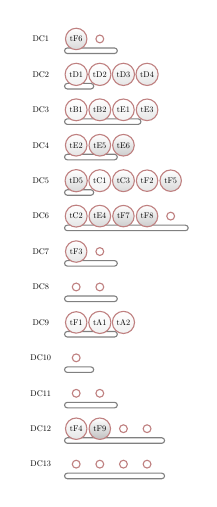
\begin{tikzpicture}[scale=0.3, every node/.style={scale=0.3}]

\tikzstyle{dc} = [rounded rectangle,right,draw=gray,yshift=-0.5cm];
\tikzstyle{task} = [circle,draw=red!50!black!50,top color=white];
\tikzstyle{dp}=[draw,opacity=0.3]
\node at (-1.5,0) {DC1};
\node[dc,text width=2.0cm] (DC1) at (-0.5,0) {};
\node[task,bottom color=black!15.0] at (0,0) {tF6};
\node[task] at (1,0) {};
\node at (-1.5,-1.5) {DC2};
\node[dc,text width=1.0cm] (DC2) at (-0.5,-1.5) {};
\node[task,bottom color=black!5.0] at (0,-1.5) {tD1};
\node[task,bottom color=black!5.0] at (1,-1.5) {tD2};
\node[task,bottom color=black!10.0] at (2,-1.5) {tD3};
\node[task,bottom color=black!10.0] at (3,-1.5) {tD4};
\node at (-1.5,-3.0) {DC3};
\node[dc,text width=3.0cm] (DC3) at (-0.5,-3.0) {};
\node[task,bottom color=black!5.0] at (0,-3.0) {tB1};
\node[task,bottom color=black!10.0] at (1,-3.0) {tB2};
\node[task,bottom color=black!5.0] at (2,-3.0) {tE1};
\node[task,bottom color=black!10.0] at (3,-3.0) {tE3};
\node at (-1.5,-4.5) {DC4};
\node[dc,text width=2.0cm] (DC4) at (-0.5,-4.5) {};
\node[task,bottom color=black!10.0] at (0,-4.5) {tE2};
\node[task,bottom color=black!15.0] at (1,-4.5) {tE5};
\node[task,bottom color=black!20.0] at (2,-4.5) {tE6};
\node at (-1.5,-6.0) {DC5};
\node[dc,text width=1.0cm] (DC5) at (-0.5,-6.0) {};
\node[task,bottom color=black!15.0] at (0,-6.0) {tD5};
\node[task,bottom color=black!5.0] at (1,-6.0) {tC1};
\node[task,bottom color=black!15.0] at (2,-6.0) {tC3};
\node[task,bottom color=black!10.0] at (3,-6.0) {tF2};
\node[task,bottom color=black!15.0] at (4,-6.0) {tF5};
\node at (-1.5,-7.5) {DC6};
\node[dc,text width=5.0cm] (DC6) at (-0.5,-7.5) {};
\node[task,bottom color=black!10.0] at (0,-7.5) {tC2};
\node[task,bottom color=black!15.0] at (1,-7.5) {tE4};
\node[task,bottom color=black!20.0] at (2,-7.5) {tF7};
\node[task,bottom color=black!20.0] at (3,-7.5) {tF8};
\node[task] at (4,-7.5) {};
\node at (-1.5,-9.0) {DC7};
\node[dc,text width=2.0cm] (DC7) at (-0.5,-9.0) {};
\node[task,bottom color=black!10.0] at (0,-9.0) {tF3};
\node[task] at (1,-9.0) {};
\node at (-1.5,-10.5) {DC8};
\node[dc,text width=2.0cm] (DC8) at (-0.5,-10.5) {};
\node[task] at (0,-10.5) {};
\node[task] at (1,-10.5) {};
\node at (-1.5,-12.0) {DC9};
\node[dc,text width=2.0cm] (DC9) at (-0.5,-12.0) {};
\node[task,bottom color=black!5.0] at (0,-12.0) {tF1};
\node[task,bottom color=black!5.0] at (1,-12.0) {tA1};
\node[task,bottom color=black!5.0] at (2,-12.0) {tA2};
\node at (-1.5,-13.5) {DC10};
\node[dc,text width=1.0cm] (DC10) at (-0.5,-13.5) {};
\node[task] at (0,-13.5) {};
\node at (-1.5,-15.0) {DC11};
\node[dc,text width=2.0cm] (DC11) at (-0.5,-15.0) {};
\node[task] at (0,-15.0) {};
\node[task] at (1,-15.0) {};
\node at (-1.5,-16.5) {DC12};
\node[dc,text width=4.0cm] (DC12) at (-0.5,-16.5) {};
\node[task,bottom color=black!10.0] at (0,-16.5) {tF4};
\node[task,bottom color=black!25.0] at (1,-16.5) {tF9};
\node[task] at (2,-16.5) {};
\node[task] at (3,-16.5) {};
\node at (-1.5,-18.0) {DC13};
\node[dc,text width=4.0cm] (DC13) at (-0.5,-18.0) {};
\node[task] at (0,-18.0) {};
\node[task] at (1,-18.0) {};
\node[task] at (2,-18.0) {};
\node[task] at (3,-18.0) {};
\end{tikzpicture}

        \end{actionenv}
        \begin{actionenv}<2->
            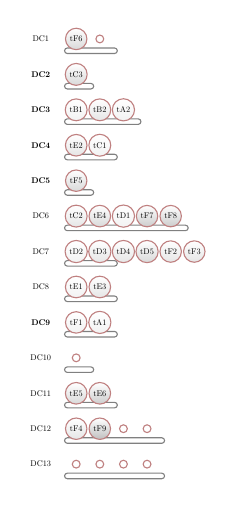
\begin{tikzpicture}[scale=0.3, every node/.style={scale=0.3}]

\tikzstyle{dc} = [rounded rectangle,right,draw=gray,yshift=-0.5cm];
\tikzstyle{task} = [circle,draw=red!50!black!50,top color=white];
\tikzstyle{dp}=[draw,opacity=0.3]
\node at (-1.5,0) {DC1};
\node[dc,text width=2.0cm] (DC1) at (-0.5,0) {};
\node[task,bottom color=black!15.0] at (0,0) {tF6};
\node[task] at (1,0) {};
\node[font=\bfseries] at (-1.5,-1.5) {DC2};
\node[dc,text width=1.0cm] (DC2) at (-0.5,-1.5) {};
\node[task,bottom color=black!15.0] at (0,-1.5) {tC3};
\node[font=\bfseries] at (-1.5,-3.0) {DC3};
\node[dc,text width=3.0cm] (DC3) at (-0.5,-3.0) {};
\node[task,bottom color=black!5.0] at (0,-3.0) {tB1};
\node[task,bottom color=black!10.0] at (1,-3.0) {tB2};
\node[task,bottom color=black!5.0] at (2,-3.0) {tA2};
\node[font=\bfseries] at (-1.5,-4.5) {DC4};
\node[dc,text width=2.0cm] (DC4) at (-0.5,-4.5) {};
\node[task,bottom color=black!10.0] at (0,-4.5) {tE2};
\node[task,bottom color=black!5.0] at (1,-4.5) {tC1};
\node[font=\bfseries] at (-1.5,-6.0) {DC5};
\node[dc,text width=1.0cm] (DC5) at (-0.5,-6.0) {};
\node[task,bottom color=black!15.0] at (0,-6.0) {tF5};
\node at (-1.5,-7.5) {DC6};
\node[dc,text width=5.0cm] (DC6) at (-0.5,-7.5) {};
\node[task,bottom color=black!10.0] at (0,-7.5) {tC2};
\node[task,bottom color=black!15.0] at (1,-7.5) {tE4};
\node[task,bottom color=black!5.0] at (2,-7.5) {tD1};
\node[task,bottom color=black!20.0] at (3,-7.5) {tF7};
\node[task,bottom color=black!20.0] at (4,-7.5) {tF8};
\node at (-1.5,-9.0) {DC7};
\node[dc,text width=2.0cm] (DC7) at (-0.5,-9.0) {};
\node[task,bottom color=black!5.0] at (0,-9.0) {tD2};
\node[task,bottom color=black!10.0] at (1,-9.0) {tD3};
\node[task,bottom color=black!10.0] at (2,-9.0) {tD4};
\node[task,bottom color=black!15.0] at (3,-9.0) {tD5};
\node[task,bottom color=black!10.0] at (4,-9.0) {tF2};
\node[task,bottom color=black!10.0] at (5,-9.0) {tF3};
\node at (-1.5,-10.5) {DC8};
\node[dc,text width=2.0cm] (DC8) at (-0.5,-10.5) {};
\node[task,bottom color=black!5.0] at (0,-10.5) {tE1};
\node[task,bottom color=black!10.0] at (1,-10.5) {tE3};
\node[font=\bfseries] at (-1.5,-12.0) {DC9};
\node[dc,text width=2.0cm] (DC9) at (-0.5,-12.0) {};
\node[task,bottom color=black!5.0] at (0,-12.0) {tF1};
\node[task,bottom color=black!5.0] at (1,-12.0) {tA1};
\node at (-1.5,-13.5) {DC10};
\node[dc,text width=1.0cm] (DC10) at (-0.5,-13.5) {};
\node[task] at (0,-13.5) {};
\node at (-1.5,-15.0) {DC11};
\node[dc,text width=2.0cm] (DC11) at (-0.5,-15.0) {};
\node[task,bottom color=black!15.0] at (0,-15.0) {tE5};
\node[task,bottom color=black!20.0] at (1,-15.0) {tE6};
\node at (-1.5,-16.5) {DC12};
\node[dc,text width=4.0cm] (DC12) at (-0.5,-16.5) {};
\node[task,bottom color=black!10.0] at (0,-16.5) {tF4};
\node[task,bottom color=black!25.0] at (1,-16.5) {tF9};
\node[task] at (2,-16.5) {};
\node[task] at (3,-16.5) {};
\node at (-1.5,-18.0) {DC13};
\node[dc,text width=4.0cm] (DC13) at (-0.5,-18.0) {};
\node[task] at (0,-18.0) {};
\node[task] at (1,-18.0) {};
\node[task] at (2,-18.0) {};
\node[task] at (3,-18.0) {};
\end{tikzpicture}

        \end{actionenv}
        \begin{actionenv}<3->
            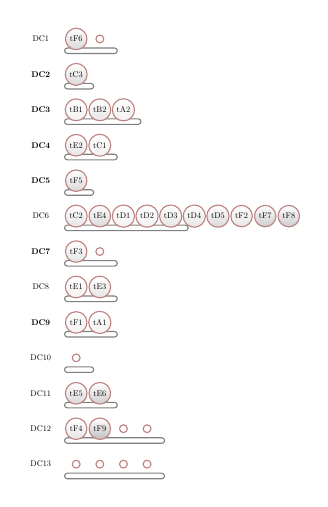
\begin{tikzpicture}[scale=0.3, every node/.style={scale=0.3}]

\tikzstyle{dc} = [rounded rectangle,right,draw=gray,yshift=-0.5cm];
\tikzstyle{task} = [circle,draw=red!50!black!50,top color=white];
\tikzstyle{dp}=[draw,opacity=0.3]
\node at (-1.5,0) {DC1};
\node[dc,text width=2.0cm] (DC1) at (-0.5,0) {};
\node[task,bottom color=black!15.0] at (0,0) {tF6};
\node[task] at (1,0) {};
\node[font=\bfseries] at (-1.5,-1.5) {DC2};
\node[dc,text width=1.0cm] (DC2) at (-0.5,-1.5) {};
\node[task,bottom color=black!15.0] at (0,-1.5) {tC3};
\node[font=\bfseries] at (-1.5,-3.0) {DC3};
\node[dc,text width=3.0cm] (DC3) at (-0.5,-3.0) {};
\node[task,bottom color=black!5.0] at (0,-3.0) {tB1};
\node[task,bottom color=black!10.0] at (1,-3.0) {tB2};
\node[task,bottom color=black!5.0] at (2,-3.0) {tA2};
\node[font=\bfseries] at (-1.5,-4.5) {DC4};
\node[dc,text width=2.0cm] (DC4) at (-0.5,-4.5) {};
\node[task,bottom color=black!10.0] at (0,-4.5) {tE2};
\node[task,bottom color=black!5.0] at (1,-4.5) {tC1};
\node[font=\bfseries] at (-1.5,-6.0) {DC5};
\node[dc,text width=1.0cm] (DC5) at (-0.5,-6.0) {};
\node[task,bottom color=black!15.0] at (0,-6.0) {tF5};
\node at (-1.5,-7.5) {DC6};
\node[dc,text width=5.0cm] (DC6) at (-0.5,-7.5) {};
\node[task,bottom color=black!10.0] at (0,-7.5) {tC2};
\node[task,bottom color=black!15.0] at (1,-7.5) {tE4};
\node[task,bottom color=black!5.0] at (2,-7.5) {tD1};
\node[task,bottom color=black!5.0] at (3,-7.5) {tD2};
\node[task,bottom color=black!10.0] at (4,-7.5) {tD3};
\node[task,bottom color=black!10.0] at (5,-7.5) {tD4};
\node[task,bottom color=black!15.0] at (6,-7.5) {tD5};
\node[task,bottom color=black!10.0] at (7,-7.5) {tF2};
\node[task,bottom color=black!20.0] at (8,-7.5) {tF7};
\node[task,bottom color=black!20.0] at (9,-7.5) {tF8};
\node[font=\bfseries] at (-1.5,-9.0) {DC7};
\node[dc,text width=2.0cm] (DC7) at (-0.5,-9.0) {};
\node[task,bottom color=black!10.0] at (0,-9.0) {tF3};
\node[task] at (1,-9.0) {};
\node at (-1.5,-10.5) {DC8};
\node[dc,text width=2.0cm] (DC8) at (-0.5,-10.5) {};
\node[task,bottom color=black!5.0] at (0,-10.5) {tE1};
\node[task,bottom color=black!10.0] at (1,-10.5) {tE3};
\node[font=\bfseries] at (-1.5,-12.0) {DC9};
\node[dc,text width=2.0cm] (DC9) at (-0.5,-12.0) {};
\node[task,bottom color=black!5.0] at (0,-12.0) {tF1};
\node[task,bottom color=black!5.0] at (1,-12.0) {tA1};
\node at (-1.5,-13.5) {DC10};
\node[dc,text width=1.0cm] (DC10) at (-0.5,-13.5) {};
\node[task] at (0,-13.5) {};
\node at (-1.5,-15.0) {DC11};
\node[dc,text width=2.0cm] (DC11) at (-0.5,-15.0) {};
\node[task,bottom color=black!15.0] at (0,-15.0) {tE5};
\node[task,bottom color=black!20.0] at (1,-15.0) {tE6};
\node at (-1.5,-16.5) {DC12};
\node[dc,text width=4.0cm] (DC12) at (-0.5,-16.5) {};
\node[task,bottom color=black!10.0] at (0,-16.5) {tF4};
\node[task,bottom color=black!25.0] at (1,-16.5) {tF9};
\node[task] at (2,-16.5) {};
\node[task] at (3,-16.5) {};
\node at (-1.5,-18.0) {DC13};
\node[dc,text width=4.0cm] (DC13) at (-0.5,-18.0) {};
\node[task] at (0,-18.0) {};
\node[task] at (1,-18.0) {};
\node[task] at (2,-18.0) {};
\node[task] at (3,-18.0) {};
\end{tikzpicture}

        \end{actionenv}
        \begin{actionenv}<4->
            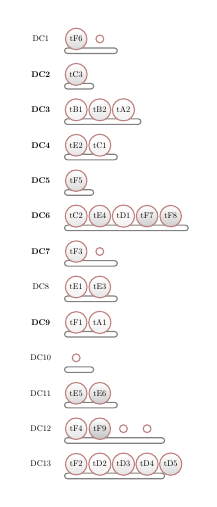
\begin{tikzpicture}[scale=0.3, every node/.style={scale=0.3}]

\tikzstyle{dc} = [rounded rectangle,right,draw=gray,yshift=-0.5cm];
\tikzstyle{task} = [circle,draw=red!50!black!50,top color=white];
\tikzstyle{dp}=[draw,opacity=0.3]
\node at (-1.5,0) {DC1};
\node[dc,text width=2.0cm] (DC1) at (-0.5,0) {};
\node[task,bottom color=black!15.0] at (0,0) {tF6};
\node[task] at (1,0) {};
\node[font=\bfseries] at (-1.5,-1.5) {DC2};
\node[dc,text width=1.0cm] (DC2) at (-0.5,-1.5) {};
\node[task,bottom color=black!15.0] at (0,-1.5) {tC3};
\node[font=\bfseries] at (-1.5,-3.0) {DC3};
\node[dc,text width=3.0cm] (DC3) at (-0.5,-3.0) {};
\node[task,bottom color=black!5.0] at (0,-3.0) {tB1};
\node[task,bottom color=black!10.0] at (1,-3.0) {tB2};
\node[task,bottom color=black!5.0] at (2,-3.0) {tA2};
\node[font=\bfseries] at (-1.5,-4.5) {DC4};
\node[dc,text width=2.0cm] (DC4) at (-0.5,-4.5) {};
\node[task,bottom color=black!10.0] at (0,-4.5) {tE2};
\node[task,bottom color=black!5.0] at (1,-4.5) {tC1};
\node[font=\bfseries] at (-1.5,-6.0) {DC5};
\node[dc,text width=1.0cm] (DC5) at (-0.5,-6.0) {};
\node[task,bottom color=black!15.0] at (0,-6.0) {tF5};
\node[font=\bfseries] at (-1.5,-7.5) {DC6};
\node[dc,text width=5.0cm] (DC6) at (-0.5,-7.5) {};
\node[task,bottom color=black!10.0] at (0,-7.5) {tC2};
\node[task,bottom color=black!15.0] at (1,-7.5) {tE4};
\node[task,bottom color=black!5.0] at (2,-7.5) {tD1};
\node[task,bottom color=black!20.0] at (3,-7.5) {tF7};
\node[task,bottom color=black!20.0] at (4,-7.5) {tF8};
\node[font=\bfseries] at (-1.5,-9.0) {DC7};
\node[dc,text width=2.0cm] (DC7) at (-0.5,-9.0) {};
\node[task,bottom color=black!10.0] at (0,-9.0) {tF3};
\node[task] at (1,-9.0) {};
\node at (-1.5,-10.5) {DC8};
\node[dc,text width=2.0cm] (DC8) at (-0.5,-10.5) {};
\node[task,bottom color=black!5.0] at (0,-10.5) {tE1};
\node[task,bottom color=black!10.0] at (1,-10.5) {tE3};
\node[font=\bfseries] at (-1.5,-12.0) {DC9};
\node[dc,text width=2.0cm] (DC9) at (-0.5,-12.0) {};
\node[task,bottom color=black!5.0] at (0,-12.0) {tF1};
\node[task,bottom color=black!5.0] at (1,-12.0) {tA1};
\node at (-1.5,-13.5) {DC10};
\node[dc,text width=1.0cm] (DC10) at (-0.5,-13.5) {};
\node[task] at (0,-13.5) {};
\node at (-1.5,-15.0) {DC11};
\node[dc,text width=2.0cm] (DC11) at (-0.5,-15.0) {};
\node[task,bottom color=black!15.0] at (0,-15.0) {tE5};
\node[task,bottom color=black!20.0] at (1,-15.0) {tE6};
\node at (-1.5,-16.5) {DC12};
\node[dc,text width=4.0cm] (DC12) at (-0.5,-16.5) {};
\node[task,bottom color=black!10.0] at (0,-16.5) {tF4};
\node[task,bottom color=black!25.0] at (1,-16.5) {tF9};
\node[task] at (2,-16.5) {};
\node[task] at (3,-16.5) {};
\node at (-1.5,-18.0) {DC13};
\node[dc,text width=4.0cm] (DC13) at (-0.5,-18.0) {};
\node[task,bottom color=black!10.0] at (0,-18.0) {tF2};
\node[task,bottom color=black!5.0] at (1,-18.0) {tD2};
\node[task,bottom color=black!10.0] at (2,-18.0) {tD3};
\node[task,bottom color=black!10.0] at (3,-18.0) {tD4};
\node[task,bottom color=black!15.0] at (4,-18.0) {tD5};
\end{tikzpicture}

        \end{actionenv}
        \begin{actionenv}<5->
            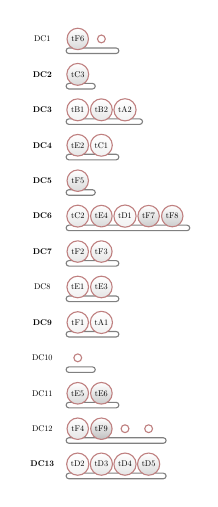
\begin{tikzpicture}[scale=0.3, every node/.style={scale=0.3}]

\tikzstyle{dc} = [rounded rectangle,right,draw=gray,yshift=-0.5cm];
\tikzstyle{task} = [circle,draw=red!50!black!50,top color=white];
\tikzstyle{dp}=[draw,opacity=0.3]
\node at (-1.5,0) {DC1};
\node[dc,text width=2.0cm] (DC1) at (-0.5,0) {};
\node[task,bottom color=black!15.0] at (0,0) {tF6};
\node[task] at (1,0) {};
\node[font=\bfseries] at (-1.5,-1.5) {DC2};
\node[dc,text width=1.0cm] (DC2) at (-0.5,-1.5) {};
\node[task,bottom color=black!15.0] at (0,-1.5) {tC3};
\node[font=\bfseries] at (-1.5,-3.0) {DC3};
\node[dc,text width=3.0cm] (DC3) at (-0.5,-3.0) {};
\node[task,bottom color=black!5.0] at (0,-3.0) {tB1};
\node[task,bottom color=black!10.0] at (1,-3.0) {tB2};
\node[task,bottom color=black!5.0] at (2,-3.0) {tA2};
\node[font=\bfseries] at (-1.5,-4.5) {DC4};
\node[dc,text width=2.0cm] (DC4) at (-0.5,-4.5) {};
\node[task,bottom color=black!10.0] at (0,-4.5) {tE2};
\node[task,bottom color=black!5.0] at (1,-4.5) {tC1};
\node[font=\bfseries] at (-1.5,-6.0) {DC5};
\node[dc,text width=1.0cm] (DC5) at (-0.5,-6.0) {};
\node[task,bottom color=black!15.0] at (0,-6.0) {tF5};
\node[font=\bfseries] at (-1.5,-7.5) {DC6};
\node[dc,text width=5.0cm] (DC6) at (-0.5,-7.5) {};
\node[task,bottom color=black!10.0] at (0,-7.5) {tC2};
\node[task,bottom color=black!15.0] at (1,-7.5) {tE4};
\node[task,bottom color=black!5.0] at (2,-7.5) {tD1};
\node[task,bottom color=black!20.0] at (3,-7.5) {tF7};
\node[task,bottom color=black!20.0] at (4,-7.5) {tF8};
\node[font=\bfseries] at (-1.5,-9.0) {DC7};
\node[dc,text width=2.0cm] (DC7) at (-0.5,-9.0) {};
\node[task,bottom color=black!10.0] at (0,-9.0) {tF2};
\node[task,bottom color=black!10.0] at (1,-9.0) {tF3};
\node at (-1.5,-10.5) {DC8};
\node[dc,text width=2.0cm] (DC8) at (-0.5,-10.5) {};
\node[task,bottom color=black!5.0] at (0,-10.5) {tE1};
\node[task,bottom color=black!10.0] at (1,-10.5) {tE3};
\node[font=\bfseries] at (-1.5,-12.0) {DC9};
\node[dc,text width=2.0cm] (DC9) at (-0.5,-12.0) {};
\node[task,bottom color=black!5.0] at (0,-12.0) {tF1};
\node[task,bottom color=black!5.0] at (1,-12.0) {tA1};
\node at (-1.5,-13.5) {DC10};
\node[dc,text width=1.0cm] (DC10) at (-0.5,-13.5) {};
\node[task] at (0,-13.5) {};
\node at (-1.5,-15.0) {DC11};
\node[dc,text width=2.0cm] (DC11) at (-0.5,-15.0) {};
\node[task,bottom color=black!15.0] at (0,-15.0) {tE5};
\node[task,bottom color=black!20.0] at (1,-15.0) {tE6};
\node at (-1.5,-16.5) {DC12};
\node[dc,text width=4.0cm] (DC12) at (-0.5,-16.5) {};
\node[task,bottom color=black!10.0] at (0,-16.5) {tF4};
\node[task,bottom color=black!25.0] at (1,-16.5) {tF9};
\node[task] at (2,-16.5) {};
\node[task] at (3,-16.5) {};
\node[font=\bfseries] at (-1.5,-18.0) {DC13};
\node[dc,text width=4.0cm] (DC13) at (-0.5,-18.0) {};
\node[task,bottom color=black!5.0] at (0,-18.0) {tD2};
\node[task,bottom color=black!10.0] at (1,-18.0) {tD3};
\node[task,bottom color=black!10.0] at (2,-18.0) {tD4};
\node[task,bottom color=black!15.0] at (3,-18.0) {tD5};
\end{tikzpicture}

        \end{actionenv}
        \caption{Iteration on Max-min Fairness}
    \end{figure}
\end{frame}

\begin{frame}
\frametitle{Toy Data Result}
    \begin{figure}
        \centering
        \begin{tikzpicture}
\begin{axis}[xlabel={iteration},
ylabel={average time},
symbolic x coords={iter.0,iter.1,iter.2,iter.3,iter.4},
width=\textwidth,
height=0.5\textheight,
xtick=data % important
]
%  \addplot+ [ybar,no markers,fill=blue!20,] coordinates { (naive,10.073)};
  \draw[red]
        (axis cs:iter.0,10.073)
        --  (axis cs:iter.4, 10.073)
    ;
 \addplot+ [ybar,no markers,fill=blue!20,] coordinates { (iter.0,9.701) (iter.1,9.854) (iter.2,10.118) (iter.3,10.301) (iter.4,10.301)};
\end{axis}
\end{tikzpicture}

        \caption{Average Time}
    \end{figure}
    The test on Toy Data indicates an average time of \textbf{10.301s} among all jobs, while maintaining max-min fairness of computing resources. The workload among all data centers are balanced.
\end{frame}

\section{Test on Real World Data}

\begin{frame}
\frametitle{Real World Data}
    Real world should satisfy that the total number of slots is larger than or equal to the total number of tasks, which means that $\sum_{i=1}^m s_i\geq \sum_{i=1}^K t_i$. In order to meet the requirement of this problem, we generate a certain amount of data sets according to certain constraints to test and check our algorithm. In our test sets, all of the data are generated by random numbers.
    
    For bandwidth, because it takes almost no time to transfer data in the same data center, its bandwidth is set to be much larger than other bandwidth values.
\end{frame}

\begin{frame}
\frametitle{Real World (without max-min)}
    \begin{figure}
        \centering
        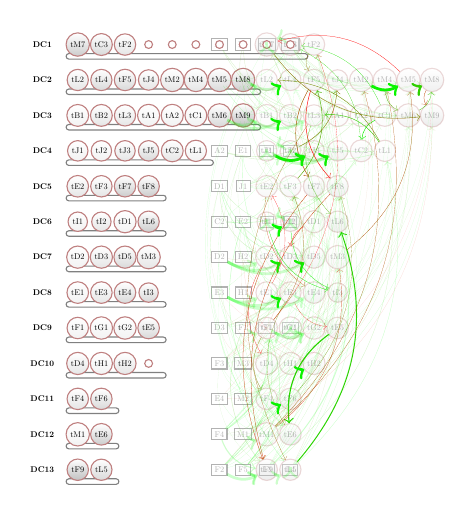
\begin{tikzpicture}[scale=0.3,every node/.style={scale=0.3}]

\tikzstyle{dc} = [rounded rectangle,right,draw=gray,yshift=-0.5cm];
\tikzstyle{task} = [circle,draw=red!50!black!50,top color=white];
\tikzstyle{dp}=[draw,opacity=0.3]
\node[font=\bfseries] at (-1.5,0) {DC1};
\node[dc,text width=10.0cm] (DC1) at (-0.5,0) {};
\node[dp] (A1) at (6,0) {A1};
\node[dp] (B1) at (7,0) {B1};
\node[dp] (M4) at (8,0) {M4};
\node[dp] (M5) at (9,0) {M5};
\node[task,bottom color=black!20.0] at (0,0) {tM7};
\node[task,bottom color=black!20.0,opacity=0.3] (tM7) at (8,0) {tM7};
\node[task,bottom color=black!15.0] at (1,0) {tC3};
\node[task,bottom color=black!15.0,opacity=0.3] (tC3) at (9,0) {tC3};
\node[task,bottom color=black!10.0] at (2,0) {tF2};
\node[task,bottom color=black!10.0,opacity=0.3] (tF2) at (10,0) {tF2};
\node[task] at (3,0) {};
\node[task] at (4,0) {};
\node[task] at (5,0) {};
\node[task] at (6,0) {};
\node[task] at (7,0) {};
\node[task] at (8,0) {};
\node[task] at (9,0) {};
\node[font=\bfseries] at (-1.5,-1.5) {DC2};
\node[dc,text width=8.0cm] (DC2) at (-0.5,-1.5) {};
\node[dp] (C1) at (6,-1.5) {C1};
\node[dp] (L2) at (7,-1.5) {L2};
\node[task,bottom color=black!10.0] at (0,-1.5) {tL2};
\node[task,bottom color=black!10.0,opacity=0.3] (tL2) at (8,-1.5) {tL2};
\node[task,bottom color=black!15.0] at (1,-1.5) {tL4};
\node[task,bottom color=black!15.0,opacity=0.3] (tL4) at (9,-1.5) {tL4};
\node[task,bottom color=black!15.0] at (2,-1.5) {tF5};
\node[task,bottom color=black!15.0,opacity=0.3] (tF5) at (10,-1.5) {tF5};
\node[task,bottom color=black!10.0] at (3,-1.5) {tJ4};
\node[task,bottom color=black!10.0,opacity=0.3] (tJ4) at (11,-1.5) {tJ4};
\node[task,bottom color=black!10.0] at (4,-1.5) {tM2};
\node[task,bottom color=black!10.0,opacity=0.3] (tM2) at (12,-1.5) {tM2};
\node[task,bottom color=black!10.0] at (5,-1.5) {tM4};
\node[task,bottom color=black!10.0,opacity=0.3] (tM4) at (13,-1.5) {tM4};
\node[task,bottom color=black!15.0] at (6,-1.5) {tM5};
\node[task,bottom color=black!15.0,opacity=0.3] (tM5) at (14,-1.5) {tM5};
\node[task,bottom color=black!20.0] at (7,-1.5) {tM8};
\node[task,bottom color=black!20.0,opacity=0.3] (tM8) at (15,-1.5) {tM8};
\node[font=\bfseries] at (-1.5,-3.0) {DC3};
\node[dc,text width=8.0cm] (DC3) at (-0.5,-3.0) {};
\node[dp] (B2) at (6,-3.0) {B2};
\node[dp] (L1) at (7,-3.0) {L1};
\node[task,bottom color=black!5.0] at (0,-3.0) {tB1};
\node[task,bottom color=black!5.0,opacity=0.3] (tB1) at (8,-3.0) {tB1};
\node[task,bottom color=black!10.0] at (1,-3.0) {tB2};
\node[task,bottom color=black!10.0,opacity=0.3] (tB2) at (9,-3.0) {tB2};
\node[task,bottom color=black!10.0] at (2,-3.0) {tL3};
\node[task,bottom color=black!10.0,opacity=0.3] (tL3) at (10,-3.0) {tL3};
\node[task,bottom color=black!5.0] at (3,-3.0) {tA1};
\node[task,bottom color=black!5.0,opacity=0.3] (tA1) at (11,-3.0) {tA1};
\node[task,bottom color=black!5.0] at (4,-3.0) {tA2};
\node[task,bottom color=black!5.0,opacity=0.3] (tA2) at (12,-3.0) {tA2};
\node[task,bottom color=black!5.0] at (5,-3.0) {tC1};
\node[task,bottom color=black!5.0,opacity=0.3] (tC1) at (13,-3.0) {tC1};
\node[task,bottom color=black!15.0] at (6,-3.0) {tM6};
\node[task,bottom color=black!15.0,opacity=0.3] (tM6) at (14,-3.0) {tM6};
\node[task,bottom color=black!25.0] at (7,-3.0) {tM9};
\node[task,bottom color=black!25.0,opacity=0.3] (tM9) at (15,-3.0) {tM9};
\node[font=\bfseries] at (-1.5,-4.5) {DC4};
\node[dc,text width=6.0cm] (DC4) at (-0.5,-4.5) {};
\node[dp] (A2) at (6,-4.5) {A2};
\node[dp] (E1) at (7,-4.5) {E1};
\node[dp] (J2) at (8,-4.5) {J2};
\node[dp] (J3) at (9,-4.5) {J3};
\node[task,bottom color=black!5.0] at (0,-4.5) {tJ1};
\node[task,bottom color=black!5.0,opacity=0.3] (tJ1) at (8,-4.5) {tJ1};
\node[task,bottom color=black!5.0] at (1,-4.5) {tJ2};
\node[task,bottom color=black!5.0,opacity=0.3] (tJ2) at (9,-4.5) {tJ2};
\node[task,bottom color=black!10.0] at (2,-4.5) {tJ3};
\node[task,bottom color=black!10.0,opacity=0.3] (tJ3) at (10,-4.5) {tJ3};
\node[task,bottom color=black!15.0] at (3,-4.5) {tJ5};
\node[task,bottom color=black!15.0,opacity=0.3] (tJ5) at (11,-4.5) {tJ5};
\node[task,bottom color=black!10.0] at (4,-4.5) {tC2};
\node[task,bottom color=black!10.0,opacity=0.3] (tC2) at (12,-4.5) {tC2};
\node[task,bottom color=black!5.0] at (5,-4.5) {tL1};
\node[task,bottom color=black!5.0,opacity=0.3] (tL1) at (13,-4.5) {tL1};
\node[font=\bfseries] at (-1.5,-6.0) {DC5};
\node[dc,text width=4.0cm] (DC5) at (-0.5,-6.0) {};
\node[dp] (D1) at (6,-6.0) {D1};
\node[dp] (J1) at (7,-6.0) {J1};
\node[task,bottom color=black!10.0] at (0,-6.0) {tE2};
\node[task,bottom color=black!10.0,opacity=0.3] (tE2) at (8,-6.0) {tE2};
\node[task,bottom color=black!10.0] at (1,-6.0) {tF3};
\node[task,bottom color=black!10.0,opacity=0.3] (tF3) at (9,-6.0) {tF3};
\node[task,bottom color=black!20.0] at (2,-6.0) {tF7};
\node[task,bottom color=black!20.0,opacity=0.3] (tF7) at (10,-6.0) {tF7};
\node[task,bottom color=black!20.0] at (3,-6.0) {tF8};
\node[task,bottom color=black!20.0,opacity=0.3] (tF8) at (11,-6.0) {tF8};
\node[font=\bfseries] at (-1.5,-7.5) {DC6};
\node[dc,text width=4.0cm] (DC6) at (-0.5,-7.5) {};
\node[dp] (C2) at (6,-7.5) {C2};
\node[dp] (E2) at (7,-7.5) {E2};
\node[dp] (I1) at (8,-7.5) {I1};
\node[dp] (I2) at (9,-7.5) {I2};
\node[task,bottom color=black!5.0] at (0,-7.5) {tI1};
\node[task,bottom color=black!5.0,opacity=0.3] (tI1) at (8,-7.5) {tI1};
\node[task,bottom color=black!10.0] at (1,-7.5) {tI2};
\node[task,bottom color=black!10.0,opacity=0.3] (tI2) at (9,-7.5) {tI2};
\node[task,bottom color=black!5.0] at (2,-7.5) {tD1};
\node[task,bottom color=black!5.0,opacity=0.3] (tD1) at (10,-7.5) {tD1};
\node[task,bottom color=black!20.0] at (3,-7.5) {tL6};
\node[task,bottom color=black!20.0,opacity=0.3] (tL6) at (11,-7.5) {tL6};
\node[font=\bfseries] at (-1.5,-9.0) {DC7};
\node[dc,text width=4.0cm] (DC7) at (-0.5,-9.0) {};
\node[dp] (D2) at (6,-9.0) {D2};
\node[dp] (H2) at (7,-9.0) {H2};
\node[task,bottom color=black!5.0] at (0,-9.0) {tD2};
\node[task,bottom color=black!5.0,opacity=0.3] (tD2) at (8,-9.0) {tD2};
\node[task,bottom color=black!10.0] at (1,-9.0) {tD3};
\node[task,bottom color=black!10.0,opacity=0.3] (tD3) at (9,-9.0) {tD3};
\node[task,bottom color=black!15.0] at (2,-9.0) {tD5};
\node[task,bottom color=black!15.0,opacity=0.3] (tD5) at (10,-9.0) {tD5};
\node[task,bottom color=black!10.0] at (3,-9.0) {tM3};
\node[task,bottom color=black!10.0,opacity=0.3] (tM3) at (11,-9.0) {tM3};
\node[font=\bfseries] at (-1.5,-10.5) {DC8};
\node[dc,text width=4.0cm] (DC8) at (-0.5,-10.5) {};
\node[dp] (E3) at (6,-10.5) {E3};
\node[dp] (H1) at (7,-10.5) {H1};
\node[task,bottom color=black!5.0] at (0,-10.5) {tE1};
\node[task,bottom color=black!5.0,opacity=0.3] (tE1) at (8,-10.5) {tE1};
\node[task,bottom color=black!10.0] at (1,-10.5) {tE3};
\node[task,bottom color=black!10.0,opacity=0.3] (tE3) at (9,-10.5) {tE3};
\node[task,bottom color=black!15.0] at (2,-10.5) {tE4};
\node[task,bottom color=black!15.0,opacity=0.3] (tE4) at (10,-10.5) {tE4};
\node[task,bottom color=black!15.0] at (3,-10.5) {tI3};
\node[task,bottom color=black!15.0,opacity=0.3] (tI3) at (11,-10.5) {tI3};
\node[font=\bfseries] at (-1.5,-12.0) {DC9};
\node[dc,text width=4.0cm] (DC9) at (-0.5,-12.0) {};
\node[dp] (D3) at (6,-12.0) {D3};
\node[dp] (F1) at (7,-12.0) {F1};
\node[dp] (G1) at (8,-12.0) {G1};
\node[dp] (G2) at (9,-12.0) {G2};
\node[task,bottom color=black!5.0] at (0,-12.0) {tF1};
\node[task,bottom color=black!5.0,opacity=0.3] (tF1) at (8,-12.0) {tF1};
\node[task,bottom color=black!5.0] at (1,-12.0) {tG1};
\node[task,bottom color=black!5.0,opacity=0.3] (tG1) at (9,-12.0) {tG1};
\node[task,bottom color=black!5.0] at (2,-12.0) {tG2};
\node[task,bottom color=black!5.0,opacity=0.3] (tG2) at (10,-12.0) {tG2};
\node[task,bottom color=black!15.0] at (3,-12.0) {tE5};
\node[task,bottom color=black!15.0,opacity=0.3] (tE5) at (11,-12.0) {tE5};
\node[font=\bfseries] at (-1.5,-13.5) {DC10};
\node[dc,text width=4.0cm] (DC10) at (-0.5,-13.5) {};
\node[dp] (F3) at (6,-13.5) {F3};
\node[dp] (M3) at (7,-13.5) {M3};
\node[task,bottom color=black!10.0] at (0,-13.5) {tD4};
\node[task,bottom color=black!10.0,opacity=0.3] (tD4) at (8,-13.5) {tD4};
\node[task,bottom color=black!5.0] at (1,-13.5) {tH1};
\node[task,bottom color=black!5.0,opacity=0.3] (tH1) at (9,-13.5) {tH1};
\node[task,bottom color=black!10.0] at (2,-13.5) {tH2};
\node[task,bottom color=black!10.0,opacity=0.3] (tH2) at (10,-13.5) {tH2};
\node[task] at (3,-13.5) {};
\node[font=\bfseries] at (-1.5,-15.0) {DC11};
\node[dc,text width=2.0cm] (DC11) at (-0.5,-15.0) {};
\node[dp] (E4) at (6,-15.0) {E4};
\node[dp] (M2) at (7,-15.0) {M2};
\node[task,bottom color=black!10.0] at (0,-15.0) {tF4};
\node[task,bottom color=black!10.0,opacity=0.3] (tF4) at (8,-15.0) {tF4};
\node[task,bottom color=black!15.0] at (1,-15.0) {tF6};
\node[task,bottom color=black!15.0,opacity=0.3] (tF6) at (9,-15.0) {tF6};
\node[font=\bfseries] at (-1.5,-16.5) {DC12};
\node[dc,text width=2.0cm] (DC12) at (-0.5,-16.5) {};
\node[dp] (F4) at (6,-16.5) {F4};
\node[dp] (M1) at (7,-16.5) {M1};
\node[task,bottom color=black!5.0] at (0,-16.5) {tM1};
\node[task,bottom color=black!5.0,opacity=0.3] (tM1) at (8,-16.5) {tM1};
\node[task,bottom color=black!20.0] at (1,-16.5) {tE6};
\node[task,bottom color=black!20.0,opacity=0.3] (tE6) at (9,-16.5) {tE6};
\node[font=\bfseries] at (-1.5,-18.0) {DC13};
\node[dc,text width=2.0cm] (DC13) at (-0.5,-18.0) {};
\node[dp] (F2) at (6,-18.0) {F2};
\node[dp] (F5) at (7,-18.0) {F5};
\node[dp] (L3) at (8,-18.0) {L3};
\node[dp] (L4) at (9,-18.0) {L4};
\node[task,bottom color=black!25.0] at (0,-18.0) {tF9};
\node[task,bottom color=black!25.0,opacity=0.3] (tF9) at (8,-18.0) {tF9};
\node[task,bottom color=black!15.0] at (1,-18.0) {tL5};
\node[task,bottom color=black!15.0,opacity=0.3] (tL5) at (9,-18.0) {tL5};
\draw[red!3.75!green,line width=1.0pt] (tB1) edge[->,bend right] (tB2);
\draw[red!6.75!green,line width=0.16666666666666666pt] (tC1) edge[->,bend right] (tC2);
\draw[red!11.25!green,line width=0.06666666666666667pt] (tC1) edge[->,bend right] (tC3);
\draw[red!15.0!green,line width=0.05pt] (tC2) edge[->,bend right] (tC3);
\draw[red!95.0!green,line width=0.07894736842105263pt] (tD1) edge[->,bend right] (tD3);
\draw[red!7.5!green,line width=1.0pt] (tD2) edge[->,bend right] (tD3);
\draw[red!100!green,line width=0.058333333333333334pt] (tD2) edge[->,bend right] (tD4);
\draw[red!7.5!green,line width=1.0pt] (tD3) edge[->,bend right] (tD5);
\draw[red!100.0!green,line width=0.0375pt] (tE1) edge[->,bend right] (tE2);
\draw[red!3.0!green,line width=1.0pt] (tE1) edge[->,bend right] (tE3);
\draw[red!80.0!green,line width=0.046875pt] (tE2) edge[->,bend right] (tE4);
\draw[red!93.825!green,line width=0.03597122302158273pt] (tE3) edge[->,bend right] (tE5);
\draw[red!46.49999999999999!green,line width=0.040322580645161296pt] (tE3) edge[->,bend right] (tE6);
\draw[red!16.2!green,line width=0.4166666666666667pt] (tE5) edge[->,bend right] (tE6);
\draw[red!100!green,line width=0.030800821355236138pt] (tF1) edge[->,bend right] (tF2);
\draw[red!65.1!green,line width=0.06912442396313365pt] (tF1) edge[->,bend right] (tF3);
\draw[red!50.0!green,line width=0.075pt] (tF1) edge[->,bend right] (tF4);
\draw[red!56.25!green,line width=0.06666666666666667pt] (tF2) edge[->,bend right] (tF5);
\draw[red!33.75!green,line width=0.16666666666666666pt] (tF3) edge[->,bend right] (tF5);
\draw[red!3.375!green,line width=1.0pt] (tF4) edge[->,bend right] (tF6);
\draw[red!67.5!green,line width=0.16666666666666666pt] (tF5) edge[->,bend right] (tF7);
\draw[red!100!green,line width=0.16666666666666666pt] (tF5) edge[->,bend right] (tF8);
\draw[red!48.75!green,line width=0.038461538461538464pt] (tF6) edge[->,bend right] (tF8);
\draw[red!78.0!green,line width=0.09615384615384616pt] (tF7) edge[->,bend right] (tF9);
\draw[red!78.0!green,line width=0.09615384615384616pt] (tF8) edge[->,bend right] (tF9);
\draw[red!3.75!green,line width=1.0pt] (tH1) edge[->,bend right] (tH2);
\draw[red!1.125!green,line width=1.0pt] (tI1) edge[->,bend right] (tI2);
\draw[red!10.0!green,line width=0.075pt] (tI1) edge[->,bend right] (tI3);
\draw[red!10.0!green,line width=0.075pt] (tI2) edge[->,bend right] (tI3);
\draw[red!7.5!green,line width=1.0pt] (tJ1) edge[->,bend right] (tJ3);
\draw[red!7.5!green,line width=1.0pt] (tJ2) edge[->,bend right] (tJ3);
\draw[red!60.0!green,line width=0.125pt] (tJ2) edge[->,bend right] (tJ4);
\draw[red!7.5!green,line width=1.0pt] (tJ3) edge[->,bend right] (tJ5);
\draw[red!45.0!green,line width=0.125pt] (tL1) edge[->,bend right] (tL2);
\draw[red!20.0!green,line width=0.15pt] (tL1) edge[->,bend right] (tL3);
\draw[red!3.75!green,line width=1.0pt] (tL2) edge[->,bend right] (tL4);
\draw[red!62.099999999999994!green,line width=0.05434782608695652pt] (tL3) edge[->,bend right] (tL5);
\draw[red!30.0!green,line width=0.0625pt] (tL3) edge[->,bend right] (tL6);
\draw[red!20.25!green,line width=0.3333333333333333pt] (tL5) edge[->,bend right] (tL6);
\draw[red!67.75000000000001!green,line width=0.05535055350553505pt] (tM1) edge[->,bend right] (tM2);
\draw[red!81.30000000000001!green,line width=0.05535055350553505pt] (tM1) edge[->,bend right] (tM3);
\draw[red!67.75000000000001!green,line width=0.05535055350553505pt] (tM1) edge[->,bend right] (tM4);
\draw[red!3.75!green,line width=1.0pt] (tM2) edge[->,bend right] (tM5);
\draw[red!67.5!green,line width=0.08333333333333333pt] (tM3) edge[->,bend right] (tM5);
\draw[red!33.75!green,line width=0.1pt] (tM4) edge[->,bend right] (tM6);
\draw[red!100!green,line width=0.08333333333333333pt] (tM5) edge[->,bend right] (tM7);
\draw[red!18.75!green,line width=1.0pt] (tM5) edge[->,bend right] (tM8);
\draw[red!22.5!green,line width=0.08333333333333333pt] (tM6) edge[->,bend right] (tM8);
\draw[red!60.0!green,line width=0.125pt] (tM7) edge[->,bend right] (tM9);
\draw[red!75.0!green,line width=0.1pt] (tM8) edge[->,bend right] (tM9);
\draw[opacity=0.2,red!25.0!green,line width=0.125pt] (A1) edge[->,bend right] (tA1);
\draw[opacity=0.2,red!25.0!green,line width=0.15pt] (A2) edge[->,bend right] (tA1);
\draw[opacity=0.2,red!25.0!green,line width=0.125pt] (A1) edge[->,bend right] (tA2);
\draw[opacity=0.2,red!25.0!green,line width=0.15pt] (A2) edge[->,bend right] (tA2);
\draw[opacity=0.2,red!30.0!green,line width=0.125pt] (B1) edge[->,bend right] (tB1);
\draw[opacity=0.2,red!3.75!green,line width=1.0pt] (B2) edge[->,bend right] (tB1);
\draw[opacity=0.2,red!33.33333333333333!green,line width=0.125pt] (B1) edge[->,bend right] (tB2);
\draw[opacity=0.2,red!6.25!green,line width=1.0pt] (B2) edge[->,bend right] (tB2);
\draw[opacity=0.2,red!10.416666666666668!green,line width=0.1pt] (C1) edge[->,bend right] (tC1);
\draw[opacity=0.2,red!11.944444444444445!green,line width=0.08720930232558138pt] (C2) edge[->,bend right] (tC1);
\draw[opacity=0.2,red!0.0!green,line width=0.13333333333333333pt] (C1) edge[->,bend right] (tC2);
\draw[opacity=0.2,red!7.000000000000001!green,line width=0.20833333333333334pt] (C2) edge[->,bend right] (tC2);
\draw[opacity=0.2,red!7.5!green,line width=0.08333333333333333pt] (C1) edge[->,bend right] (tC3);
\draw[opacity=0.2,red!0.0!green,line width=0.040540540540540536pt] (C2) edge[->,bend right] (tC3);
\draw[opacity=0.2,red!16.666666666666664!green,line width=0.125pt] (D1) edge[->,bend right] (tD1);
\draw[opacity=0.2,red!58.333333333333336!green,line width=0.07142857142857142pt] (D2) edge[->,bend right] (tD1);
\draw[opacity=0.2,red!48.75000000000001!green,line width=0.1282051282051282pt] (D3) edge[->,bend right] (tD1);
\draw[opacity=0.2,red!25.0!green,line width=0.16666666666666666pt] (D1) edge[->,bend right] (tD2);
\draw[opacity=0.2,red!6.25!green,line width=1.0pt] (D2) edge[->,bend right] (tD2);
\draw[opacity=0.2,red!42.63888888888889!green,line width=0.048859934853420196pt] (D3) edge[->,bend right] (tD2);
\draw[opacity=0.2,red!0.0!green,line width=0.16666666666666666pt] (D1) edge[->,bend right] (tD3);
\draw[opacity=0.2,red!1.0416666666666665!green,line width=1.0pt] (D2) edge[->,bend right] (tD3);
\draw[opacity=0.2,red!0.0!green,line width=0.048859934853420196pt] (D3) edge[->,bend right] (tD3);
\draw[opacity=0.2,red!48.21428571428571!green,line width=0.04320987654320988pt] (D1) edge[->,bend right] (tD4);
\draw[opacity=0.2,red!0.0!green,line width=0.058333333333333334pt] (D2) edge[->,bend right] (tD4);
\draw[opacity=0.2,red!71.80555555555556!green,line width=0.029013539651837526pt] (D3) edge[->,bend right] (tD4);
\draw[opacity=0.2,red!0.0!green,line width=0.16666666666666666pt] (D1) edge[->,bend right] (tD5);
\draw[opacity=0.2,red!4.166666666666666!green,line width=1.0pt] (D2) edge[->,bend right] (tD5);
\draw[opacity=0.2,red!0.0!green,line width=0.048859934853420196pt] (D3) edge[->,bend right] (tD5);
\draw[opacity=0.2,red!29.166666666666664!green,line width=0.04285714285714286pt] (E1) edge[->,bend right] (tE1);
\draw[opacity=0.2,red!22.22222222222222!green,line width=0.075pt] (E2) edge[->,bend right] (tE1);
\draw[opacity=0.2,red!2.5!green,line width=1.0pt] (E3) edge[->,bend right] (tE1);
\draw[opacity=0.2,red!0.0!green,line width=0.023076923076923075pt] (E4) edge[->,bend right] (tE1);
\draw[opacity=0.2,red!0.0!green,line width=0.07142857142857142pt] (E1) edge[->,bend right] (tE2);
\draw[opacity=0.2,red!12.5!green,line width=0.15pt] (E2) edge[->,bend right] (tE2);
\draw[opacity=0.2,red!0.0!green,line width=0.0375pt] (E3) edge[->,bend right] (tE2);
\draw[opacity=0.2,red!65.0!green,line width=0.038461538461538464pt] (E4) edge[->,bend right] (tE2);
\draw[opacity=0.2,red!14.583333333333332!green,line width=0.04285714285714286pt] (E1) edge[->,bend right] (tE3);
\draw[opacity=0.2,red!0.0!green,line width=0.075pt] (E2) edge[->,bend right] (tE3);
\draw[opacity=0.2,red!1.0416666666666665!green,line width=1.0pt] (E3) edge[->,bend right] (tE3);
\draw[opacity=0.2,red!0.0!green,line width=0.023076923076923075pt] (E4) edge[->,bend right] (tE3);
\draw[opacity=0.2,red!0.0!green,line width=0.04285714285714286pt] (E1) edge[->,bend right] (tE4);
\draw[opacity=0.2,red!44.44444444444444!green,line width=0.075pt] (E2) edge[->,bend right] (tE4);
\draw[opacity=0.2,red!0.0!green,line width=1.0pt] (E3) edge[->,bend right] (tE4);
\draw[opacity=0.2,red!0.0!green,line width=0.023076923076923075pt] (E4) edge[->,bend right] (tE4);
\draw[opacity=0.2,red!0.0!green,line width=0.05617977528089888pt] (E1) edge[->,bend right] (tE5);
\draw[opacity=0.2,red!0.0!green,line width=0.1282051282051282pt] (E2) edge[->,bend right] (tE5);
\draw[opacity=0.2,red!92.66666666666666!green,line width=0.03597122302158273pt] (E3) edge[->,bend right] (tE5);
\draw[opacity=0.2,red!90.0!green,line width=0.041666666666666664pt] (E4) edge[->,bend right] (tE5);
\draw[opacity=0.2,red!15.416666666666668!green,line width=0.06756756756756757pt] (E1) edge[->,bend right] (tE6);
\draw[opacity=0.2,red!0.0!green,line width=0.20833333333333334pt] (E2) edge[->,bend right] (tE6);
\draw[opacity=0.2,red!0.0!green,line width=0.040322580645161296pt] (E3) edge[->,bend right] (tE6);
\draw[opacity=0.2,red!0.0!green,line width=0.03787878787878789pt] (E4) edge[->,bend right] (tE6);
\draw[opacity=0.2,red!6.25!green,line width=1.0pt] (F1) edge[->,bend right] (tF1);
\draw[opacity=0.2,red!0.0!green,line width=0.18518518518518517pt] (F2) edge[->,bend right] (tF1);
\draw[opacity=0.2,red!0.0!green,line width=0.025678650036683785pt] (F3) edge[->,bend right] (tF1);
\draw[opacity=0.2,red!0.0!green,line width=0.3333333333333333pt] (F4) edge[->,bend right] (tF1);
\draw[opacity=0.2,red!0.0!green,line width=0.18518518518518517pt] (F5) edge[->,bend right] (tF1);
\draw[opacity=0.2,red!0.0!green,line width=0.030800821355236138pt] (F1) edge[->,bend right] (tF2);
\draw[opacity=0.2,red!57.63888888888889!green,line width=0.03614457831325301pt] (F2) edge[->,bend right] (tF2);
\draw[opacity=0.2,red!0.0!green,line width=0.024305555555555552pt] (F3) edge[->,bend right] (tF2);
\draw[opacity=0.2,red!0.0!green,line width=0.03325942350332595pt] (F4) edge[->,bend right] (tF2);
\draw[opacity=0.2,red!0.0!green,line width=0.03614457831325301pt] (F5) edge[->,bend right] (tF2);
\draw[opacity=0.2,red!0.0!green,line width=0.06912442396313365pt] (F1) edge[->,bend right] (tF3);
\draw[opacity=0.2,red!0.0!green,line width=0.10344827586206896pt] (F2) edge[->,bend right] (tF3);
\draw[opacity=0.2,red!96.42857142857142!green,line width=0.04320987654320988pt] (F3) edge[->,bend right] (tF3);
\draw[opacity=0.2,red!0.0!green,line width=0.08287292817679558pt] (F4) edge[->,bend right] (tF3);
\draw[opacity=0.2,red!0.0!green,line width=0.10344827586206896pt] (F5) edge[->,bend right] (tF3);
\draw[opacity=0.2,red!0.0!green,line width=0.075pt] (F1) edge[->,bend right] (tF4);
\draw[opacity=0.2,red!0.0!green,line width=0.05338078291814946pt] (F2) edge[->,bend right] (tF4);
\draw[opacity=0.2,red!0.0!green,line width=0.021212121212121213pt] (F3) edge[->,bend right] (tF4);
\draw[opacity=0.2,red!34.02777777777778!green,line width=0.06122448979591836pt] (F4) edge[->,bend right] (tF4);
\draw[opacity=0.2,red!0.0!green,line width=0.05338078291814946pt] (F5) edge[->,bend right] (tF4);
\draw[opacity=0.2,red!21.319444444444446!green,line width=0.048859934853420196pt] (F1) edge[->,bend right] (tF5);
\draw[opacity=0.2,red!16.319444444444446!green,line width=0.06382978723404255pt] (F2) edge[->,bend right] (tF5);
\draw[opacity=0.2,red!30.357142857142854!green,line width=0.03431372549019608pt] (F3) edge[->,bend right] (tF5);
\draw[opacity=0.2,red!0.0!green,line width=0.05535055350553505pt] (F4) edge[->,bend right] (tF5);
\draw[opacity=0.2,red!0.0!green,line width=0.06382978723404255pt] (F5) edge[->,bend right] (tF5);
\draw[opacity=0.2,red!19.444444444444446!green,line width=0.075pt] (F1) edge[->,bend right] (tF6);
\draw[opacity=0.2,red!0.0!green,line width=0.05338078291814946pt] (F2) edge[->,bend right] (tF6);
\draw[opacity=0.2,red!0.0!green,line width=0.021212121212121213pt] (F3) edge[->,bend right] (tF6);
\draw[opacity=0.2,red!23.819444444444446!green,line width=0.06122448979591836pt] (F4) edge[->,bend right] (tF6);
\draw[opacity=0.2,red!0.0!green,line width=0.05338078291814946pt] (F5) edge[->,bend right] (tF6);
\draw[opacity=0.2,red!0.0!green,line width=0.06912442396313365pt] (F1) edge[->,bend right] (tF7);
\draw[opacity=0.2,red!0.0!green,line width=0.10344827586206896pt] (F2) edge[->,bend right] (tF7);
\draw[opacity=0.2,red!48.21428571428571!green,line width=0.04320987654320988pt] (F3) edge[->,bend right] (tF7);
\draw[opacity=0.2,red!0.0!green,line width=0.08287292817679558pt] (F4) edge[->,bend right] (tF7);
\draw[opacity=0.2,red!40.27777777777778!green,line width=0.10344827586206896pt] (F5) edge[->,bend right] (tF7);
\draw[opacity=0.2,red!0.0!green,line width=0.06912442396313365pt] (F1) edge[->,bend right] (tF8);
\draw[opacity=0.2,red!30.208333333333332!green,line width=0.10344827586206896pt] (F2) edge[->,bend right] (tF8);
\draw[opacity=0.2,red!0.0!green,line width=0.04320987654320988pt] (F3) edge[->,bend right] (tF8);
\draw[opacity=0.2,red!0.0!green,line width=0.08287292817679558pt] (F4) edge[->,bend right] (tF8);
\draw[opacity=0.2,red!20.13888888888889!green,line width=0.10344827586206896pt] (F5) edge[->,bend right] (tF8);
\draw[opacity=0.2,red!25.0!green,line width=0.20833333333333334pt] (F1) edge[->,bend right] (tF9);
\draw[opacity=0.2,red!0.0!green,line width=1.0pt] (F2) edge[->,bend right] (tF9);
\draw[opacity=0.2,red!20.96428571428571!green,line width=0.02981260647359455pt] (F3) edge[->,bend right] (tF9);
\draw[opacity=0.2,red!4.0!green,line width=0.4166666666666667pt] (F4) edge[->,bend right] (tF9);
\draw[opacity=0.2,red!4.166666666666666!green,line width=1.0pt] (F5) edge[->,bend right] (tF9);
\draw[opacity=0.2,red!3.125!green,line width=1.0pt] (G1) edge[->,bend right] (tG1);
\draw[opacity=0.2,red!3.75!green,line width=1.0pt] (G2) edge[->,bend right] (tG1);
\draw[opacity=0.2,red!3.125!green,line width=1.0pt] (G1) edge[->,bend right] (tG2);
\draw[opacity=0.2,red!3.75!green,line width=1.0pt] (G2) edge[->,bend right] (tG2);
\draw[opacity=0.2,red!50.0!green,line width=0.075pt] (H1) edge[->,bend right] (tH1);
\draw[opacity=0.2,red!64.28571428571429!green,line width=0.058333333333333334pt] (H2) edge[->,bend right] (tH1);
\draw[opacity=0.2,red!55.55555555555556!green,line width=0.075pt] (H1) edge[->,bend right] (tH2);
\draw[opacity=0.2,red!100!green,line width=0.058333333333333334pt] (H2) edge[->,bend right] (tH2);
\draw[opacity=0.2,red!1.0416666666666665!green,line width=1.0pt] (I1) edge[->,bend right] (tI1);
\draw[opacity=0.2,red!1.0416666666666665!green,line width=1.0pt] (I2) edge[->,bend right] (tI1);
\draw[opacity=0.2,red!0.0!green,line width=1.0pt] (I1) edge[->,bend right] (tI2);
\draw[opacity=0.2,red!1.4583333333333333!green,line width=1.0pt] (I2) edge[->,bend right] (tI2);
\draw[opacity=0.2,red!8.333333333333332!green,line width=0.075pt] (I1) edge[->,bend right] (tI3);
\draw[opacity=0.2,red!0.0!green,line width=0.075pt] (I2) edge[->,bend right] (tI3);
\draw[opacity=0.2,red!26.66666666666667!green,line width=0.07812499999999999pt] (J1) edge[->,bend right] (tJ1);
\draw[opacity=0.2,red!4.166666666666666!green,line width=1.0pt] (J2) edge[->,bend right] (tJ1);
\draw[opacity=0.2,red!6.25!green,line width=1.0pt] (J3) edge[->,bend right] (tJ1);
\draw[opacity=0.2,red!53.33333333333334!green,line width=0.07812499999999999pt] (J1) edge[->,bend right] (tJ2);
\draw[opacity=0.2,red!6.25!green,line width=1.0pt] (J2) edge[->,bend right] (tJ2);
\draw[opacity=0.2,red!2.083333333333333!green,line width=1.0pt] (J3) edge[->,bend right] (tJ2);
\draw[opacity=0.2,red!0.0!green,line width=0.07812499999999999pt] (J1) edge[->,bend right] (tJ3);
\draw[opacity=0.2,red!1.0416666666666665!green,line width=1.0pt] (J2) edge[->,bend right] (tJ3);
\draw[opacity=0.2,red!0.0!green,line width=1.0pt] (J3) edge[->,bend right] (tJ3);
\draw[opacity=0.2,red!12.5!green,line width=0.16666666666666666pt] (J1) edge[->,bend right] (tJ4);
\draw[opacity=0.2,red!0.0!green,line width=0.125pt] (J2) edge[->,bend right] (tJ4);
\draw[opacity=0.2,red!16.666666666666664!green,line width=0.125pt] (J3) edge[->,bend right] (tJ4);
\draw[opacity=0.2,red!0.0!green,line width=0.07812499999999999pt] (J1) edge[->,bend right] (tJ5);
\draw[opacity=0.2,red!4.166666666666666!green,line width=1.0pt] (J2) edge[->,bend right] (tJ5);
\draw[opacity=0.2,red!0.0!green,line width=1.0pt] (J3) edge[->,bend right] (tJ5);
\draw[opacity=0.2,red!7.5!green,line width=0.16666666666666666pt] (L1) edge[->,bend right] (tL1);
\draw[opacity=0.2,red!12.5!green,line width=0.13333333333333333pt] (L2) edge[->,bend right] (tL1);
\draw[opacity=0.2,red!19.5!green,line width=0.1282051282051282pt] (L3) edge[->,bend right] (tL1);
\draw[opacity=0.2,red!0.0!green,line width=0.1282051282051282pt] (L4) edge[->,bend right] (tL1);
\draw[opacity=0.2,red!0.0!green,line width=0.08333333333333333pt] (L1) edge[->,bend right] (tL2);
\draw[opacity=0.2,red!1.875!green,line width=1.0pt] (L2) edge[->,bend right] (tL2);
\draw[opacity=0.2,red!0.0!green,line width=0.06382978723404255pt] (L3) edge[->,bend right] (tL2);
\draw[opacity=0.2,red!39.16666666666667!green,line width=0.06382978723404255pt] (L4) edge[->,bend right] (tL2);
\draw[opacity=0.2,red!0.625!green,line width=1.0pt] (L1) edge[->,bend right] (tL3);
\draw[opacity=0.2,red!0.0!green,line width=0.1pt] (L2) edge[->,bend right] (tL3);
\draw[opacity=0.2,red!15.069444444444446!green,line width=0.06912442396313363pt] (L3) edge[->,bend right] (tL3);
\draw[opacity=0.2,red!0.0!green,line width=0.06912442396313363pt] (L4) edge[->,bend right] (tL3);
\draw[opacity=0.2,red!0.0!green,line width=0.08333333333333333pt] (L1) edge[->,bend right] (tL4);
\draw[opacity=0.2,red!3.3333333333333335!green,line width=1.0pt] (L2) edge[->,bend right] (tL4);
\draw[opacity=0.2,red!0.0!green,line width=0.06382978723404255pt] (L3) edge[->,bend right] (tL4);
\draw[opacity=0.2,red!0.0!green,line width=0.06382978723404255pt] (L4) edge[->,bend right] (tL4);
\draw[opacity=0.2,red!0.0!green,line width=0.05434782608695652pt] (L1) edge[->,bend right] (tL5);
\draw[opacity=0.2,red!0.0!green,line width=0.06097560975609756pt] (L2) edge[->,bend right] (tL5);
\draw[opacity=0.2,red!3.3333333333333335!green,line width=1.0pt] (L3) edge[->,bend right] (tL5);
\draw[opacity=0.2,red!3.75!green,line width=1.0pt] (L4) edge[->,bend right] (tL5);
\draw[opacity=0.2,red!16.666666666666664!green,line width=0.0625pt] (L1) edge[->,bend right] (tL6);
\draw[opacity=0.2,red!0.0!green,line width=0.07142857142857142pt] (L2) edge[->,bend right] (tL6);
\draw[opacity=0.2,red!0.0!green,line width=0.3333333333333333pt] (L3) edge[->,bend right] (tL6);
\draw[opacity=0.2,red!0.0!green,line width=0.3333333333333333pt] (L4) edge[->,bend right] (tL6);
\draw[opacity=0.2,red!6.25!green,line width=1.0pt] (M1) edge[->,bend right] (tM1);
\draw[opacity=0.2,red!0.0!green,line width=0.03787878787878789pt] (M2) edge[->,bend right] (tM1);
\draw[opacity=0.2,red!0.0!green,line width=0.02782193958664547pt] (M3) edge[->,bend right] (tM1);
\draw[opacity=0.2,red!0.0!green,line width=0.03472222222222222pt] (M4) edge[->,bend right] (tM1);
\draw[opacity=0.2,red!0.0!green,line width=0.03472222222222222pt] (M5) edge[->,bend right] (tM1);
\draw[opacity=0.2,red!0.0!green,line width=0.05535055350553505pt] (M1) edge[->,bend right] (tM2);
\draw[opacity=0.2,red!66.66666666666666!green,line width=0.03125pt] (M2) edge[->,bend right] (tM2);
\draw[opacity=0.2,red!0.0!green,line width=0.03431372549019608pt] (M3) edge[->,bend right] (tM2);
\draw[opacity=0.2,red!0.0!green,line width=0.06666666666666667pt] (M4) edge[->,bend right] (tM2);
\draw[opacity=0.2,red!0.0!green,line width=0.06666666666666667pt] (M5) edge[->,bend right] (tM2);
\draw[opacity=0.2,red!0.0!green,line width=0.05535055350553505pt] (M1) edge[->,bend right] (tM3);
\draw[opacity=0.2,red!0.0!green,line width=0.05pt] (M2) edge[->,bend right] (tM3);
\draw[opacity=0.2,red!71.42857142857143!green,line width=0.058333333333333334pt] (M3) edge[->,bend right] (tM3);
\draw[opacity=0.2,red!0.0!green,line width=0.03703703703703703pt] (M4) edge[->,bend right] (tM3);
\draw[opacity=0.2,red!0.0!green,line width=0.03703703703703703pt] (M5) edge[->,bend right] (tM3);
\draw[opacity=0.2,red!0.0!green,line width=0.05535055350553505pt] (M1) edge[->,bend right] (tM4);
\draw[opacity=0.2,red!0.0!green,line width=0.03125pt] (M2) edge[->,bend right] (tM4);
\draw[opacity=0.2,red!0.0!green,line width=0.03431372549019608pt] (M3) edge[->,bend right] (tM4);
\draw[opacity=0.2,red!31.25!green,line width=0.06666666666666667pt] (M4) edge[->,bend right] (tM4);
\draw[opacity=0.2,red!0.0!green,line width=0.06666666666666667pt] (M5) edge[->,bend right] (tM4);
\draw[opacity=0.2,red!18.819444444444446!green,line width=0.05535055350553505pt] (M1) edge[->,bend right] (tM5);
\draw[opacity=0.2,red!33.33333333333333!green,line width=0.03125pt] (M2) edge[->,bend right] (tM5);
\draw[opacity=0.2,red!30.357142857142854!green,line width=0.03431372549019608pt] (M3) edge[->,bend right] (tM5);
\draw[opacity=0.2,red!0.0!green,line width=0.06666666666666667pt] (M4) edge[->,bend right] (tM5);
\draw[opacity=0.2,red!0.0!green,line width=0.06666666666666667pt] (M5) edge[->,bend right] (tM5);
\draw[opacity=0.2,red!24.59722222222222!green,line width=0.05928853754940711pt] (M1) edge[->,bend right] (tM6);
\draw[opacity=0.2,red!0.0!green,line width=0.02411575562700964pt] (M2) edge[->,bend right] (tM6);
\draw[opacity=0.2,red!0.0!green,line width=0.025547445255474453pt] (M3) edge[->,bend right] (tM6);
\draw[opacity=0.2,red!11.666666666666666!green,line width=0.125pt] (M4) edge[->,bend right] (tM6);
\draw[opacity=0.2,red!0.0!green,line width=0.125pt] (M5) edge[->,bend right] (tM6);
\draw[opacity=0.2,red!0.0!green,line width=0.03325942350332595pt] (M1) edge[->,bend right] (tM7);
\draw[opacity=0.2,red!0.0!green,line width=0.022727272727272728pt] (M2) edge[->,bend right] (tM7);
\draw[opacity=0.2,red!85.71428571428572!green,line width=0.024305555555555552pt] (M3) edge[->,bend right] (tM7);
\draw[opacity=0.2,red!0.0!green,line width=1.0pt] (M4) edge[->,bend right] (tM7);
\draw[opacity=0.2,red!4.166666666666666!green,line width=1.0pt] (M5) edge[->,bend right] (tM7);
\draw[opacity=0.2,red!0.0!green,line width=0.05535055350553505pt] (M1) edge[->,bend right] (tM8);
\draw[opacity=0.2,red!100.0!green,line width=0.03125pt] (M2) edge[->,bend right] (tM8);
\draw[opacity=0.2,red!0.0!green,line width=0.03431372549019608pt] (M3) edge[->,bend right] (tM8);
\draw[opacity=0.2,red!0.0!green,line width=0.06666666666666667pt] (M4) edge[->,bend right] (tM8);
\draw[opacity=0.2,red!31.25!green,line width=0.06666666666666667pt] (M5) edge[->,bend right] (tM8);
\draw[opacity=0.2,red!87.84722222222223!green,line width=0.05928853754940711pt] (M1) edge[->,bend right] (tM9);
\draw[opacity=0.2,red!0.0!green,line width=0.02411575562700964pt] (M2) edge[->,bend right] (tM9);
\draw[opacity=0.2,red!24.46428571428571!green,line width=0.025547445255474453pt] (M3) edge[->,bend right] (tM9);
\draw[opacity=0.2,red!13.333333333333334!green,line width=0.125pt] (M4) edge[->,bend right] (tM9);
\draw[opacity=0.2,red!33.33333333333333!green,line width=0.125pt] (M5) edge[->,bend right] (tM9);
\end{tikzpicture}

        \caption{Real World Allocation without max-min}
    \end{figure}
\end{frame}

\begin{frame}
\frametitle{Real World (max-min iteration)}
    \begin{figure}[h]
        \centering
        \begin{actionenv}<1->
            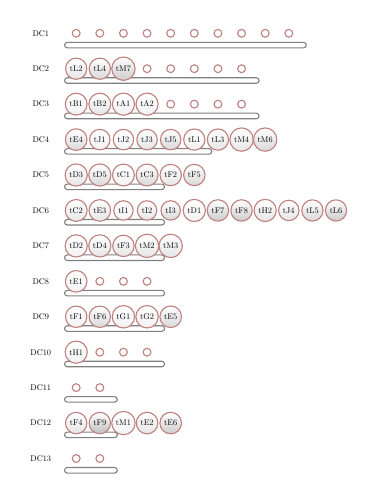
\begin{tikzpicture}[scale=0.3, every node/.style={scale=0.3}]

\tikzstyle{dc} = [rounded rectangle,right,draw=gray,yshift=-0.5cm];
\tikzstyle{task} = [circle,draw=red!50!black!50,top color=white];
\tikzstyle{dp}=[draw,opacity=0.3]
\node at (-1.5,0) {DC1};
\node[dc,text width=10.0cm] (DC1) at (-0.5,0) {};
\node[task] at (0,0) {};
\node[task] at (1,0) {};
\node[task] at (2,0) {};
\node[task] at (3,0) {};
\node[task] at (4,0) {};
\node[task] at (5,0) {};
\node[task] at (6,0) {};
\node[task] at (7,0) {};
\node[task] at (8,0) {};
\node[task] at (9,0) {};
\node at (-1.5,-1.5) {DC2};
\node[dc,text width=8.0cm] (DC2) at (-0.5,-1.5) {};
\node[task,bottom color=black!10.0] at (0,-1.5) {tL2};
\node[task,bottom color=black!15.0] at (1,-1.5) {tL4};
\node[task,bottom color=black!20.0] at (2,-1.5) {tM7};
\node[task] at (3,-1.5) {};
\node[task] at (4,-1.5) {};
\node[task] at (5,-1.5) {};
\node[task] at (6,-1.5) {};
\node[task] at (7,-1.5) {};
\node at (-1.5,-3.0) {DC3};
\node[dc,text width=8.0cm] (DC3) at (-0.5,-3.0) {};
\node[task,bottom color=black!5.0] at (0,-3.0) {tB1};
\node[task,bottom color=black!10.0] at (1,-3.0) {tB2};
\node[task,bottom color=black!5.0] at (2,-3.0) {tA1};
\node[task,bottom color=black!5.0] at (3,-3.0) {tA2};
\node[task] at (4,-3.0) {};
\node[task] at (5,-3.0) {};
\node[task] at (6,-3.0) {};
\node[task] at (7,-3.0) {};
\node at (-1.5,-4.5) {DC4};
\node[dc,text width=6.0cm] (DC4) at (-0.5,-4.5) {};
\node[task,bottom color=black!15.0] at (0,-4.5) {tE4};
\node[task,bottom color=black!5.0] at (1,-4.5) {tJ1};
\node[task,bottom color=black!5.0] at (2,-4.5) {tJ2};
\node[task,bottom color=black!10.0] at (3,-4.5) {tJ3};
\node[task,bottom color=black!15.0] at (4,-4.5) {tJ5};
\node[task,bottom color=black!5.0] at (5,-4.5) {tL1};
\node[task,bottom color=black!10.0] at (6,-4.5) {tL3};
\node[task,bottom color=black!10.0] at (7,-4.5) {tM4};
\node[task,bottom color=black!15.0] at (8,-4.5) {tM6};
\node at (-1.5,-6.0) {DC5};
\node[dc,text width=4.0cm] (DC5) at (-0.5,-6.0) {};
\node[task,bottom color=black!10.0] at (0,-6.0) {tD3};
\node[task,bottom color=black!15.0] at (1,-6.0) {tD5};
\node[task,bottom color=black!5.0] at (2,-6.0) {tC1};
\node[task,bottom color=black!15.0] at (3,-6.0) {tC3};
\node[task,bottom color=black!10.0] at (4,-6.0) {tF2};
\node[task,bottom color=black!15.0] at (5,-6.0) {tF5};
\node at (-1.5,-7.5) {DC6};
\node[dc,text width=4.0cm] (DC6) at (-0.5,-7.5) {};
\node[task,bottom color=black!10.0] at (0,-7.5) {tC2};
\node[task,bottom color=black!10.0] at (1,-7.5) {tE3};
\node[task,bottom color=black!5.0] at (2,-7.5) {tI1};
\node[task,bottom color=black!10.0] at (3,-7.5) {tI2};
\node[task,bottom color=black!15.0] at (4,-7.5) {tI3};
\node[task,bottom color=black!5.0] at (5,-7.5) {tD1};
\node[task,bottom color=black!20.0] at (6,-7.5) {tF7};
\node[task,bottom color=black!20.0] at (7,-7.5) {tF8};
\node[task,bottom color=black!10.0] at (8,-7.5) {tH2};
\node[task,bottom color=black!10.0] at (9,-7.5) {tJ4};
\node[task,bottom color=black!15.0] at (10,-7.5) {tL5};
\node[task,bottom color=black!20.0] at (11,-7.5) {tL6};
\node at (-1.5,-9.0) {DC7};
\node[dc,text width=4.0cm] (DC7) at (-0.5,-9.0) {};
\node[task,bottom color=black!5.0] at (0,-9.0) {tD2};
\node[task,bottom color=black!10.0] at (1,-9.0) {tD4};
\node[task,bottom color=black!10.0] at (2,-9.0) {tF3};
\node[task,bottom color=black!10.0] at (3,-9.0) {tM2};
\node[task,bottom color=black!10.0] at (4,-9.0) {tM3};
\node at (-1.5,-10.5) {DC8};
\node[dc,text width=4.0cm] (DC8) at (-0.5,-10.5) {};
\node[task,bottom color=black!5.0] at (0,-10.5) {tE1};
\node[task] at (1,-10.5) {};
\node[task] at (2,-10.5) {};
\node[task] at (3,-10.5) {};
\node at (-1.5,-12.0) {DC9};
\node[dc,text width=4.0cm] (DC9) at (-0.5,-12.0) {};
\node[task,bottom color=black!5.0] at (0,-12.0) {tF1};
\node[task,bottom color=black!15.0] at (1,-12.0) {tF6};
\node[task,bottom color=black!5.0] at (2,-12.0) {tG1};
\node[task,bottom color=black!5.0] at (3,-12.0) {tG2};
\node[task,bottom color=black!15.0] at (4,-12.0) {tE5};
\node at (-1.5,-13.5) {DC10};
\node[dc,text width=4.0cm] (DC10) at (-0.5,-13.5) {};
\node[task,bottom color=black!5.0] at (0,-13.5) {tH1};
\node[task] at (1,-13.5) {};
\node[task] at (2,-13.5) {};
\node[task] at (3,-13.5) {};
\node at (-1.5,-15.0) {DC11};
\node[dc,text width=2.0cm] (DC11) at (-0.5,-15.0) {};
\node[task] at (0,-15.0) {};
\node[task] at (1,-15.0) {};
\node at (-1.5,-16.5) {DC12};
\node[dc,text width=2.0cm] (DC12) at (-0.5,-16.5) {};
\node[task,bottom color=black!10.0] at (0,-16.5) {tF4};
\node[task,bottom color=black!25.0] at (1,-16.5) {tF9};
\node[task,bottom color=black!5.0] at (2,-16.5) {tM1};
\node[task,bottom color=black!10.0] at (3,-16.5) {tE2};
\node[task,bottom color=black!20.0] at (4,-16.5) {tE6};
\node at (-1.5,-18.0) {DC13};
\node[dc,text width=2.0cm] (DC13) at (-0.5,-18.0) {};
\node[task] at (0,-18.0) {};
\node[task] at (1,-18.0) {};
\end{tikzpicture}

        \end{actionenv}
        \begin{actionenv}<2->
            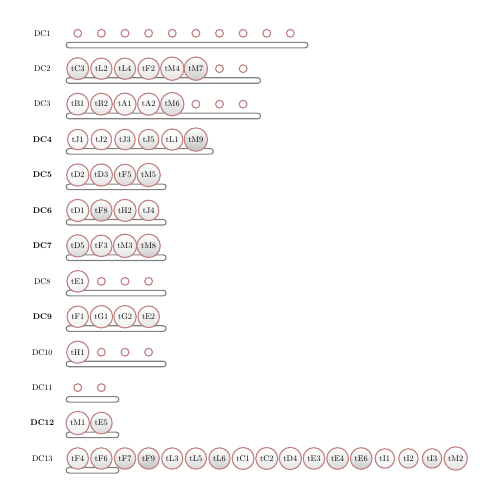
\begin{tikzpicture}[scale=0.3, every node/.style={scale=0.3}]

\tikzstyle{dc} = [rounded rectangle,right,draw=gray,yshift=-0.5cm];
\tikzstyle{task} = [circle,draw=red!50!black!50,top color=white];
\tikzstyle{dp}=[draw,opacity=0.3]
\node at (-1.5,0) {DC1};
\node[dc,text width=10.0cm] (DC1) at (-0.5,0) {};
\node[task] at (0,0) {};
\node[task] at (1,0) {};
\node[task] at (2,0) {};
\node[task] at (3,0) {};
\node[task] at (4,0) {};
\node[task] at (5,0) {};
\node[task] at (6,0) {};
\node[task] at (7,0) {};
\node[task] at (8,0) {};
\node[task] at (9,0) {};
\node at (-1.5,-1.5) {DC2};
\node[dc,text width=8.0cm] (DC2) at (-0.5,-1.5) {};
\node[task,bottom color=black!15.0] at (0,-1.5) {tC3};
\node[task,bottom color=black!10.0] at (1,-1.5) {tL2};
\node[task,bottom color=black!15.0] at (2,-1.5) {tL4};
\node[task,bottom color=black!10.0] at (3,-1.5) {tF2};
\node[task,bottom color=black!10.0] at (4,-1.5) {tM4};
\node[task,bottom color=black!20.0] at (5,-1.5) {tM7};
\node[task] at (6,-1.5) {};
\node[task] at (7,-1.5) {};
\node at (-1.5,-3.0) {DC3};
\node[dc,text width=8.0cm] (DC3) at (-0.5,-3.0) {};
\node[task,bottom color=black!5.0] at (0,-3.0) {tB1};
\node[task,bottom color=black!10.0] at (1,-3.0) {tB2};
\node[task,bottom color=black!5.0] at (2,-3.0) {tA1};
\node[task,bottom color=black!5.0] at (3,-3.0) {tA2};
\node[task,bottom color=black!15.0] at (4,-3.0) {tM6};
\node[task] at (5,-3.0) {};
\node[task] at (6,-3.0) {};
\node[task] at (7,-3.0) {};
\node[font=\bfseries] at (-1.5,-4.5) {DC4};
\node[dc,text width=6.0cm] (DC4) at (-0.5,-4.5) {};
\node[task,bottom color=black!5.0] at (0,-4.5) {tJ1};
\node[task,bottom color=black!5.0] at (1,-4.5) {tJ2};
\node[task,bottom color=black!10.0] at (2,-4.5) {tJ3};
\node[task,bottom color=black!15.0] at (3,-4.5) {tJ5};
\node[task,bottom color=black!5.0] at (4,-4.5) {tL1};
\node[task,bottom color=black!25.0] at (5,-4.5) {tM9};
\node[font=\bfseries] at (-1.5,-6.0) {DC5};
\node[dc,text width=4.0cm] (DC5) at (-0.5,-6.0) {};
\node[task,bottom color=black!5.0] at (0,-6.0) {tD2};
\node[task,bottom color=black!10.0] at (1,-6.0) {tD3};
\node[task,bottom color=black!15.0] at (2,-6.0) {tF5};
\node[task,bottom color=black!15.0] at (3,-6.0) {tM5};
\node[font=\bfseries] at (-1.5,-7.5) {DC6};
\node[dc,text width=4.0cm] (DC6) at (-0.5,-7.5) {};
\node[task,bottom color=black!5.0] at (0,-7.5) {tD1};
\node[task,bottom color=black!20.0] at (1,-7.5) {tF8};
\node[task,bottom color=black!10.0] at (2,-7.5) {tH2};
\node[task,bottom color=black!10.0] at (3,-7.5) {tJ4};
\node[font=\bfseries] at (-1.5,-9.0) {DC7};
\node[dc,text width=4.0cm] (DC7) at (-0.5,-9.0) {};
\node[task,bottom color=black!15.0] at (0,-9.0) {tD5};
\node[task,bottom color=black!10.0] at (1,-9.0) {tF3};
\node[task,bottom color=black!10.0] at (2,-9.0) {tM3};
\node[task,bottom color=black!20.0] at (3,-9.0) {tM8};
\node at (-1.5,-10.5) {DC8};
\node[dc,text width=4.0cm] (DC8) at (-0.5,-10.5) {};
\node[task,bottom color=black!5.0] at (0,-10.5) {tE1};
\node[task] at (1,-10.5) {};
\node[task] at (2,-10.5) {};
\node[task] at (3,-10.5) {};
\node[font=\bfseries] at (-1.5,-12.0) {DC9};
\node[dc,text width=4.0cm] (DC9) at (-0.5,-12.0) {};
\node[task,bottom color=black!5.0] at (0,-12.0) {tF1};
\node[task,bottom color=black!5.0] at (1,-12.0) {tG1};
\node[task,bottom color=black!5.0] at (2,-12.0) {tG2};
\node[task,bottom color=black!10.0] at (3,-12.0) {tE2};
\node at (-1.5,-13.5) {DC10};
\node[dc,text width=4.0cm] (DC10) at (-0.5,-13.5) {};
\node[task,bottom color=black!5.0] at (0,-13.5) {tH1};
\node[task] at (1,-13.5) {};
\node[task] at (2,-13.5) {};
\node[task] at (3,-13.5) {};
\node at (-1.5,-15.0) {DC11};
\node[dc,text width=2.0cm] (DC11) at (-0.5,-15.0) {};
\node[task] at (0,-15.0) {};
\node[task] at (1,-15.0) {};
\node[font=\bfseries] at (-1.5,-16.5) {DC12};
\node[dc,text width=2.0cm] (DC12) at (-0.5,-16.5) {};
\node[task,bottom color=black!5.0] at (0,-16.5) {tM1};
\node[task,bottom color=black!15.0] at (1,-16.5) {tE5};
\node at (-1.5,-18.0) {DC13};
\node[dc,text width=2.0cm] (DC13) at (-0.5,-18.0) {};
\node[task,bottom color=black!10.0] at (0,-18.0) {tF4};
\node[task,bottom color=black!15.0] at (1,-18.0) {tF6};
\node[task,bottom color=black!20.0] at (2,-18.0) {tF7};
\node[task,bottom color=black!25.0] at (3,-18.0) {tF9};
\node[task,bottom color=black!10.0] at (4,-18.0) {tL3};
\node[task,bottom color=black!15.0] at (5,-18.0) {tL5};
\node[task,bottom color=black!20.0] at (6,-18.0) {tL6};
\node[task,bottom color=black!5.0] at (7,-18.0) {tC1};
\node[task,bottom color=black!10.0] at (8,-18.0) {tC2};
\node[task,bottom color=black!10.0] at (9,-18.0) {tD4};
\node[task,bottom color=black!10.0] at (10,-18.0) {tE3};
\node[task,bottom color=black!15.0] at (11,-18.0) {tE4};
\node[task,bottom color=black!20.0] at (12,-18.0) {tE6};
\node[task,bottom color=black!5.0] at (13,-18.0) {tI1};
\node[task,bottom color=black!10.0] at (14,-18.0) {tI2};
\node[task,bottom color=black!15.0] at (15,-18.0) {tI3};
\node[task,bottom color=black!10.0] at (16,-18.0) {tM2};
\end{tikzpicture}

        \end{actionenv}
        \caption{Iteration on Max-min Fairness}
    \end{figure}
\end{frame}

\begin{frame}
\frametitle{Real World (max-min iteration)}
    \begin{figure}[h]
        \centering
        \begin{actionenv}<1->
            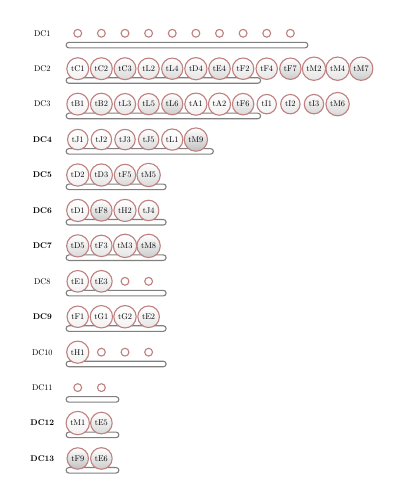
\begin{tikzpicture}[scale=0.3, every node/.style={scale=0.3}]

\tikzstyle{dc} = [rounded rectangle,right,draw=gray,yshift=-0.5cm];
\tikzstyle{task} = [circle,draw=red!50!black!50,top color=white];
\tikzstyle{dp}=[draw,opacity=0.3]
\node at (-1.5,0) {DC1};
\node[dc,text width=10.0cm] (DC1) at (-0.5,0) {};
\node[task] at (0,0) {};
\node[task] at (1,0) {};
\node[task] at (2,0) {};
\node[task] at (3,0) {};
\node[task] at (4,0) {};
\node[task] at (5,0) {};
\node[task] at (6,0) {};
\node[task] at (7,0) {};
\node[task] at (8,0) {};
\node[task] at (9,0) {};
\node at (-1.5,-1.5) {DC2};
\node[dc,text width=8.0cm] (DC2) at (-0.5,-1.5) {};
\node[task,bottom color=black!5.0] at (0,-1.5) {tC1};
\node[task,bottom color=black!10.0] at (1,-1.5) {tC2};
\node[task,bottom color=black!15.0] at (2,-1.5) {tC3};
\node[task,bottom color=black!10.0] at (3,-1.5) {tL2};
\node[task,bottom color=black!15.0] at (4,-1.5) {tL4};
\node[task,bottom color=black!10.0] at (5,-1.5) {tD4};
\node[task,bottom color=black!15.0] at (6,-1.5) {tE4};
\node[task,bottom color=black!10.0] at (7,-1.5) {tF2};
\node[task,bottom color=black!10.0] at (8,-1.5) {tF4};
\node[task,bottom color=black!20.0] at (9,-1.5) {tF7};
\node[task,bottom color=black!10.0] at (10,-1.5) {tM2};
\node[task,bottom color=black!10.0] at (11,-1.5) {tM4};
\node[task,bottom color=black!20.0] at (12,-1.5) {tM7};
\node at (-1.5,-3.0) {DC3};
\node[dc,text width=8.0cm] (DC3) at (-0.5,-3.0) {};
\node[task,bottom color=black!5.0] at (0,-3.0) {tB1};
\node[task,bottom color=black!10.0] at (1,-3.0) {tB2};
\node[task,bottom color=black!10.0] at (2,-3.0) {tL3};
\node[task,bottom color=black!15.0] at (3,-3.0) {tL5};
\node[task,bottom color=black!20.0] at (4,-3.0) {tL6};
\node[task,bottom color=black!5.0] at (5,-3.0) {tA1};
\node[task,bottom color=black!5.0] at (6,-3.0) {tA2};
\node[task,bottom color=black!15.0] at (7,-3.0) {tF6};
\node[task,bottom color=black!5.0] at (8,-3.0) {tI1};
\node[task,bottom color=black!10.0] at (9,-3.0) {tI2};
\node[task,bottom color=black!15.0] at (10,-3.0) {tI3};
\node[task,bottom color=black!15.0] at (11,-3.0) {tM6};
\node[font=\bfseries] at (-1.5,-4.5) {DC4};
\node[dc,text width=6.0cm] (DC4) at (-0.5,-4.5) {};
\node[task,bottom color=black!5.0] at (0,-4.5) {tJ1};
\node[task,bottom color=black!5.0] at (1,-4.5) {tJ2};
\node[task,bottom color=black!10.0] at (2,-4.5) {tJ3};
\node[task,bottom color=black!15.0] at (3,-4.5) {tJ5};
\node[task,bottom color=black!5.0] at (4,-4.5) {tL1};
\node[task,bottom color=black!25.0] at (5,-4.5) {tM9};
\node[font=\bfseries] at (-1.5,-6.0) {DC5};
\node[dc,text width=4.0cm] (DC5) at (-0.5,-6.0) {};
\node[task,bottom color=black!5.0] at (0,-6.0) {tD2};
\node[task,bottom color=black!10.0] at (1,-6.0) {tD3};
\node[task,bottom color=black!15.0] at (2,-6.0) {tF5};
\node[task,bottom color=black!15.0] at (3,-6.0) {tM5};
\node[font=\bfseries] at (-1.5,-7.5) {DC6};
\node[dc,text width=4.0cm] (DC6) at (-0.5,-7.5) {};
\node[task,bottom color=black!5.0] at (0,-7.5) {tD1};
\node[task,bottom color=black!20.0] at (1,-7.5) {tF8};
\node[task,bottom color=black!10.0] at (2,-7.5) {tH2};
\node[task,bottom color=black!10.0] at (3,-7.5) {tJ4};
\node[font=\bfseries] at (-1.5,-9.0) {DC7};
\node[dc,text width=4.0cm] (DC7) at (-0.5,-9.0) {};
\node[task,bottom color=black!15.0] at (0,-9.0) {tD5};
\node[task,bottom color=black!10.0] at (1,-9.0) {tF3};
\node[task,bottom color=black!10.0] at (2,-9.0) {tM3};
\node[task,bottom color=black!20.0] at (3,-9.0) {tM8};
\node at (-1.5,-10.5) {DC8};
\node[dc,text width=4.0cm] (DC8) at (-0.5,-10.5) {};
\node[task,bottom color=black!5.0] at (0,-10.5) {tE1};
\node[task,bottom color=black!10.0] at (1,-10.5) {tE3};
\node[task] at (2,-10.5) {};
\node[task] at (3,-10.5) {};
\node[font=\bfseries] at (-1.5,-12.0) {DC9};
\node[dc,text width=4.0cm] (DC9) at (-0.5,-12.0) {};
\node[task,bottom color=black!5.0] at (0,-12.0) {tF1};
\node[task,bottom color=black!5.0] at (1,-12.0) {tG1};
\node[task,bottom color=black!5.0] at (2,-12.0) {tG2};
\node[task,bottom color=black!10.0] at (3,-12.0) {tE2};
\node at (-1.5,-13.5) {DC10};
\node[dc,text width=4.0cm] (DC10) at (-0.5,-13.5) {};
\node[task,bottom color=black!5.0] at (0,-13.5) {tH1};
\node[task] at (1,-13.5) {};
\node[task] at (2,-13.5) {};
\node[task] at (3,-13.5) {};
\node at (-1.5,-15.0) {DC11};
\node[dc,text width=2.0cm] (DC11) at (-0.5,-15.0) {};
\node[task] at (0,-15.0) {};
\node[task] at (1,-15.0) {};
\node[font=\bfseries] at (-1.5,-16.5) {DC12};
\node[dc,text width=2.0cm] (DC12) at (-0.5,-16.5) {};
\node[task,bottom color=black!5.0] at (0,-16.5) {tM1};
\node[task,bottom color=black!15.0] at (1,-16.5) {tE5};
\node[font=\bfseries] at (-1.5,-18.0) {DC13};
\node[dc,text width=2.0cm] (DC13) at (-0.5,-18.0) {};
\node[task,bottom color=black!25.0] at (0,-18.0) {tF9};
\node[task,bottom color=black!20.0] at (1,-18.0) {tE6};
\end{tikzpicture}

        \end{actionenv}
        \begin{actionenv}<2->
            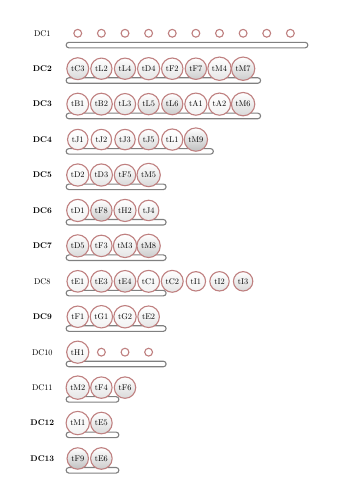
\begin{tikzpicture}[scale=0.3, every node/.style={scale=0.3}]

\tikzstyle{dc} = [rounded rectangle,right,draw=gray,yshift=-0.5cm];
\tikzstyle{task} = [circle,draw=red!50!black!50,top color=white];
\tikzstyle{dp}=[draw,opacity=0.3]
\node at (-1.5,0) {DC1};
\node[dc,text width=10.0cm] (DC1) at (-0.5,0) {};
\node[task] at (0,0) {};
\node[task] at (1,0) {};
\node[task] at (2,0) {};
\node[task] at (3,0) {};
\node[task] at (4,0) {};
\node[task] at (5,0) {};
\node[task] at (6,0) {};
\node[task] at (7,0) {};
\node[task] at (8,0) {};
\node[task] at (9,0) {};
\node[font=\bfseries] at (-1.5,-1.5) {DC2};
\node[dc,text width=8.0cm] (DC2) at (-0.5,-1.5) {};
\node[task,bottom color=black!15.0] at (0,-1.5) {tC3};
\node[task,bottom color=black!10.0] at (1,-1.5) {tL2};
\node[task,bottom color=black!15.0] at (2,-1.5) {tL4};
\node[task,bottom color=black!10.0] at (3,-1.5) {tD4};
\node[task,bottom color=black!10.0] at (4,-1.5) {tF2};
\node[task,bottom color=black!20.0] at (5,-1.5) {tF7};
\node[task,bottom color=black!10.0] at (6,-1.5) {tM4};
\node[task,bottom color=black!20.0] at (7,-1.5) {tM7};
\node[font=\bfseries] at (-1.5,-3.0) {DC3};
\node[dc,text width=8.0cm] (DC3) at (-0.5,-3.0) {};
\node[task,bottom color=black!5.0] at (0,-3.0) {tB1};
\node[task,bottom color=black!10.0] at (1,-3.0) {tB2};
\node[task,bottom color=black!10.0] at (2,-3.0) {tL3};
\node[task,bottom color=black!15.0] at (3,-3.0) {tL5};
\node[task,bottom color=black!20.0] at (4,-3.0) {tL6};
\node[task,bottom color=black!5.0] at (5,-3.0) {tA1};
\node[task,bottom color=black!5.0] at (6,-3.0) {tA2};
\node[task,bottom color=black!15.0] at (7,-3.0) {tM6};
\node[font=\bfseries] at (-1.5,-4.5) {DC4};
\node[dc,text width=6.0cm] (DC4) at (-0.5,-4.5) {};
\node[task,bottom color=black!5.0] at (0,-4.5) {tJ1};
\node[task,bottom color=black!5.0] at (1,-4.5) {tJ2};
\node[task,bottom color=black!10.0] at (2,-4.5) {tJ3};
\node[task,bottom color=black!15.0] at (3,-4.5) {tJ5};
\node[task,bottom color=black!5.0] at (4,-4.5) {tL1};
\node[task,bottom color=black!25.0] at (5,-4.5) {tM9};
\node[font=\bfseries] at (-1.5,-6.0) {DC5};
\node[dc,text width=4.0cm] (DC5) at (-0.5,-6.0) {};
\node[task,bottom color=black!5.0] at (0,-6.0) {tD2};
\node[task,bottom color=black!10.0] at (1,-6.0) {tD3};
\node[task,bottom color=black!15.0] at (2,-6.0) {tF5};
\node[task,bottom color=black!15.0] at (3,-6.0) {tM5};
\node[font=\bfseries] at (-1.5,-7.5) {DC6};
\node[dc,text width=4.0cm] (DC6) at (-0.5,-7.5) {};
\node[task,bottom color=black!5.0] at (0,-7.5) {tD1};
\node[task,bottom color=black!20.0] at (1,-7.5) {tF8};
\node[task,bottom color=black!10.0] at (2,-7.5) {tH2};
\node[task,bottom color=black!10.0] at (3,-7.5) {tJ4};
\node[font=\bfseries] at (-1.5,-9.0) {DC7};
\node[dc,text width=4.0cm] (DC7) at (-0.5,-9.0) {};
\node[task,bottom color=black!15.0] at (0,-9.0) {tD5};
\node[task,bottom color=black!10.0] at (1,-9.0) {tF3};
\node[task,bottom color=black!10.0] at (2,-9.0) {tM3};
\node[task,bottom color=black!20.0] at (3,-9.0) {tM8};
\node at (-1.5,-10.5) {DC8};
\node[dc,text width=4.0cm] (DC8) at (-0.5,-10.5) {};
\node[task,bottom color=black!5.0] at (0,-10.5) {tE1};
\node[task,bottom color=black!10.0] at (1,-10.5) {tE3};
\node[task,bottom color=black!15.0] at (2,-10.5) {tE4};
\node[task,bottom color=black!5.0] at (3,-10.5) {tC1};
\node[task,bottom color=black!10.0] at (4,-10.5) {tC2};
\node[task,bottom color=black!5.0] at (5,-10.5) {tI1};
\node[task,bottom color=black!10.0] at (6,-10.5) {tI2};
\node[task,bottom color=black!15.0] at (7,-10.5) {tI3};
\node[font=\bfseries] at (-1.5,-12.0) {DC9};
\node[dc,text width=4.0cm] (DC9) at (-0.5,-12.0) {};
\node[task,bottom color=black!5.0] at (0,-12.0) {tF1};
\node[task,bottom color=black!5.0] at (1,-12.0) {tG1};
\node[task,bottom color=black!5.0] at (2,-12.0) {tG2};
\node[task,bottom color=black!10.0] at (3,-12.0) {tE2};
\node at (-1.5,-13.5) {DC10};
\node[dc,text width=4.0cm] (DC10) at (-0.5,-13.5) {};
\node[task,bottom color=black!5.0] at (0,-13.5) {tH1};
\node[task] at (1,-13.5) {};
\node[task] at (2,-13.5) {};
\node[task] at (3,-13.5) {};
\node at (-1.5,-15.0) {DC11};
\node[dc,text width=2.0cm] (DC11) at (-0.5,-15.0) {};
\node[task,bottom color=black!10.0] at (0,-15.0) {tM2};
\node[task,bottom color=black!10.0] at (1,-15.0) {tF4};
\node[task,bottom color=black!15.0] at (2,-15.0) {tF6};
\node[font=\bfseries] at (-1.5,-16.5) {DC12};
\node[dc,text width=2.0cm] (DC12) at (-0.5,-16.5) {};
\node[task,bottom color=black!5.0] at (0,-16.5) {tM1};
\node[task,bottom color=black!15.0] at (1,-16.5) {tE5};
\node[font=\bfseries] at (-1.5,-18.0) {DC13};
\node[dc,text width=2.0cm] (DC13) at (-0.5,-18.0) {};
\node[task,bottom color=black!25.0] at (0,-18.0) {tF9};
\node[task,bottom color=black!20.0] at (1,-18.0) {tE6};
\end{tikzpicture}

        \end{actionenv}
        \begin{actionenv}<3->
            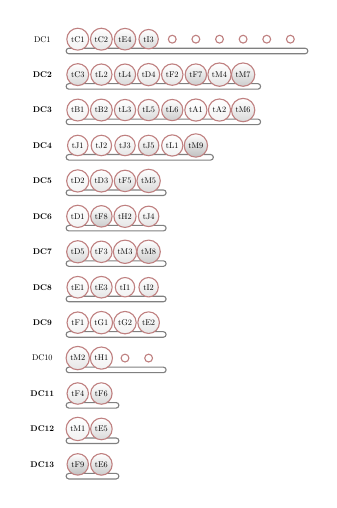
\begin{tikzpicture}[scale=0.3, every node/.style={scale=0.3}]

\tikzstyle{dc} = [rounded rectangle,right,draw=gray,yshift=-0.5cm];
\tikzstyle{task} = [circle,draw=red!50!black!50,top color=white];
\tikzstyle{dp}=[draw,opacity=0.3]
\node at (-1.5,0) {DC1};
\node[dc,text width=10.0cm] (DC1) at (-0.5,0) {};
\node[task,bottom color=black!5.0] at (0,0) {tC1};
\node[task,bottom color=black!10.0] at (1,0) {tC2};
\node[task,bottom color=black!15.0] at (2,0) {tE4};
\node[task,bottom color=black!15.0] at (3,0) {tI3};
\node[task] at (4,0) {};
\node[task] at (5,0) {};
\node[task] at (6,0) {};
\node[task] at (7,0) {};
\node[task] at (8,0) {};
\node[task] at (9,0) {};
\node[font=\bfseries] at (-1.5,-1.5) {DC2};
\node[dc,text width=8.0cm] (DC2) at (-0.5,-1.5) {};
\node[task,bottom color=black!15.0] at (0,-1.5) {tC3};
\node[task,bottom color=black!10.0] at (1,-1.5) {tL2};
\node[task,bottom color=black!15.0] at (2,-1.5) {tL4};
\node[task,bottom color=black!10.0] at (3,-1.5) {tD4};
\node[task,bottom color=black!10.0] at (4,-1.5) {tF2};
\node[task,bottom color=black!20.0] at (5,-1.5) {tF7};
\node[task,bottom color=black!10.0] at (6,-1.5) {tM4};
\node[task,bottom color=black!20.0] at (7,-1.5) {tM7};
\node[font=\bfseries] at (-1.5,-3.0) {DC3};
\node[dc,text width=8.0cm] (DC3) at (-0.5,-3.0) {};
\node[task,bottom color=black!5.0] at (0,-3.0) {tB1};
\node[task,bottom color=black!10.0] at (1,-3.0) {tB2};
\node[task,bottom color=black!10.0] at (2,-3.0) {tL3};
\node[task,bottom color=black!15.0] at (3,-3.0) {tL5};
\node[task,bottom color=black!20.0] at (4,-3.0) {tL6};
\node[task,bottom color=black!5.0] at (5,-3.0) {tA1};
\node[task,bottom color=black!5.0] at (6,-3.0) {tA2};
\node[task,bottom color=black!15.0] at (7,-3.0) {tM6};
\node[font=\bfseries] at (-1.5,-4.5) {DC4};
\node[dc,text width=6.0cm] (DC4) at (-0.5,-4.5) {};
\node[task,bottom color=black!5.0] at (0,-4.5) {tJ1};
\node[task,bottom color=black!5.0] at (1,-4.5) {tJ2};
\node[task,bottom color=black!10.0] at (2,-4.5) {tJ3};
\node[task,bottom color=black!15.0] at (3,-4.5) {tJ5};
\node[task,bottom color=black!5.0] at (4,-4.5) {tL1};
\node[task,bottom color=black!25.0] at (5,-4.5) {tM9};
\node[font=\bfseries] at (-1.5,-6.0) {DC5};
\node[dc,text width=4.0cm] (DC5) at (-0.5,-6.0) {};
\node[task,bottom color=black!5.0] at (0,-6.0) {tD2};
\node[task,bottom color=black!10.0] at (1,-6.0) {tD3};
\node[task,bottom color=black!15.0] at (2,-6.0) {tF5};
\node[task,bottom color=black!15.0] at (3,-6.0) {tM5};
\node[font=\bfseries] at (-1.5,-7.5) {DC6};
\node[dc,text width=4.0cm] (DC6) at (-0.5,-7.5) {};
\node[task,bottom color=black!5.0] at (0,-7.5) {tD1};
\node[task,bottom color=black!20.0] at (1,-7.5) {tF8};
\node[task,bottom color=black!10.0] at (2,-7.5) {tH2};
\node[task,bottom color=black!10.0] at (3,-7.5) {tJ4};
\node[font=\bfseries] at (-1.5,-9.0) {DC7};
\node[dc,text width=4.0cm] (DC7) at (-0.5,-9.0) {};
\node[task,bottom color=black!15.0] at (0,-9.0) {tD5};
\node[task,bottom color=black!10.0] at (1,-9.0) {tF3};
\node[task,bottom color=black!10.0] at (2,-9.0) {tM3};
\node[task,bottom color=black!20.0] at (3,-9.0) {tM8};
\node[font=\bfseries] at (-1.5,-10.5) {DC8};
\node[dc,text width=4.0cm] (DC8) at (-0.5,-10.5) {};
\node[task,bottom color=black!5.0] at (0,-10.5) {tE1};
\node[task,bottom color=black!10.0] at (1,-10.5) {tE3};
\node[task,bottom color=black!5.0] at (2,-10.5) {tI1};
\node[task,bottom color=black!10.0] at (3,-10.5) {tI2};
\node[font=\bfseries] at (-1.5,-12.0) {DC9};
\node[dc,text width=4.0cm] (DC9) at (-0.5,-12.0) {};
\node[task,bottom color=black!5.0] at (0,-12.0) {tF1};
\node[task,bottom color=black!5.0] at (1,-12.0) {tG1};
\node[task,bottom color=black!5.0] at (2,-12.0) {tG2};
\node[task,bottom color=black!10.0] at (3,-12.0) {tE2};
\node at (-1.5,-13.5) {DC10};
\node[dc,text width=4.0cm] (DC10) at (-0.5,-13.5) {};
\node[task,bottom color=black!10.0] at (0,-13.5) {tM2};
\node[task,bottom color=black!5.0] at (1,-13.5) {tH1};
\node[task] at (2,-13.5) {};
\node[task] at (3,-13.5) {};
\node[font=\bfseries] at (-1.5,-15.0) {DC11};
\node[dc,text width=2.0cm] (DC11) at (-0.5,-15.0) {};
\node[task,bottom color=black!10.0] at (0,-15.0) {tF4};
\node[task,bottom color=black!15.0] at (1,-15.0) {tF6};
\node[font=\bfseries] at (-1.5,-16.5) {DC12};
\node[dc,text width=2.0cm] (DC12) at (-0.5,-16.5) {};
\node[task,bottom color=black!5.0] at (0,-16.5) {tM1};
\node[task,bottom color=black!15.0] at (1,-16.5) {tE5};
\node[font=\bfseries] at (-1.5,-18.0) {DC13};
\node[dc,text width=2.0cm] (DC13) at (-0.5,-18.0) {};
\node[task,bottom color=black!25.0] at (0,-18.0) {tF9};
\node[task,bottom color=black!20.0] at (1,-18.0) {tE6};
\end{tikzpicture}

        \end{actionenv}
        \caption{Iteration on Max-min Fairness}
    \end{figure}
\end{frame}

\begin{frame}
\frametitle{Running Time}
The running time is 15s, which indicates that our algorithm is efficient enough. While the algorithm without max-min is 10min.
\end{frame}

% 我认为可以到这里结束了,代码演示一下

\end{document}